% The entire content of this work (including the source code
% for TeX files and the generated PDF documents) by 
% Hongxiang Chen (nicknamed we.taper, or just Taper) is
% licensed under a 
% Creative Commons Attribution-NonCommercial-ShareAlike 4.0 
% International License (Link to the complete license text:
% http://creativecommons.org/licenses/by-nc-sa/4.0/).
\documentclass{article}

% My own physics package
% The following line load the package xparse with additional option to
% prevent the annoying warnings, which are caused by the package
% "physics" loaded in package "physicist-taper".
\usepackage[log-declarations=false]{xparse}
\usepackage{physicist-taper}

\makenomenclature

% Show the keys for labels, replace options with "final" when done
% with editing.
\usepackage[draft,notref]{showkeys}

\pdfoptionpdfminorversion=7
\title{Notes of Basic Topolgy}
\date{\today}
\author{Taper}


\begin{document}


\maketitle
\abstract{
    A note of Basic Topology, based on \textit{Basic Topology} by M.A.
    Armstrong.
}
\tableofcontents
There are several parts that I will skipped for convenience. Those
include chapter 1 - Introduction, chapter 2 - Continuity, chapter 3 -
Compactness and Connectedness, and chapter 4 - Identification Spaces.
Below is some especially confusing part that I would like to note:

\section{Special Notes}
\label{sec:Special-Notes}

\paragraph{About map} In book \cite{book}, a map is defined as a
continuous function (page 32), which is confusing. In this note, I
will not use this convention and will always states continuity
clearly.

\paragraph{Basic facts about maps}
Assuming domain $f=X$, codomain $f=Y$.
\begin{align}
    f(U\cup V) &= f(U)\cup f(V) \\
    f(U\cap V) &\subseteq f(U)\cap f(V) \\
    f(U^c) &\supseteq f(U)^c,\,\text{i.e. } f(U)^c \subseteq f(U^c) \\
    f^{-1}(U\cup V) &= f^{-1}(U)\cup f^{-1}(V) \\
    f^{-1}(U\cap V) &= f^{-1}(U)\cap f^{-1}(V) \\
    f^{-1}(U^c) &= [f^{-1}(U)]^c
\end{align}
\paragraph{Smallest the Largest Topolgy}
The set of all possible topolgies on $X$ is partially ordered by
inclusion. For a certain characteristics $\mathcal{C}$, it is possible
to have the smallest or the largest one. 

The \nomen{smallest topolgy} $\mathcal{T}_\text{min}$ is the one such
that, for any $\mathcal{T}'$ satisfying $\mathcal{C}$,
$\mathcal{T}_\text{min}\subseteq \mathcal{T}'$. The \nomen{largest
topolgy} $\mathcal{T}_\text{max}$ is the one such that, for any
$\mathcal{T}'$ satisfying $\mathcal{C}$, $\mathcal{T}'\subseteq
\mathcal{T}_\text{max}$.
Synonyms of these two words are:
\begin{itemize}
    \item Larger: stronger, finer.
    \item Smaller: weaker, coarser.
\end{itemize}
\begin{figure}[H]
    \centering
    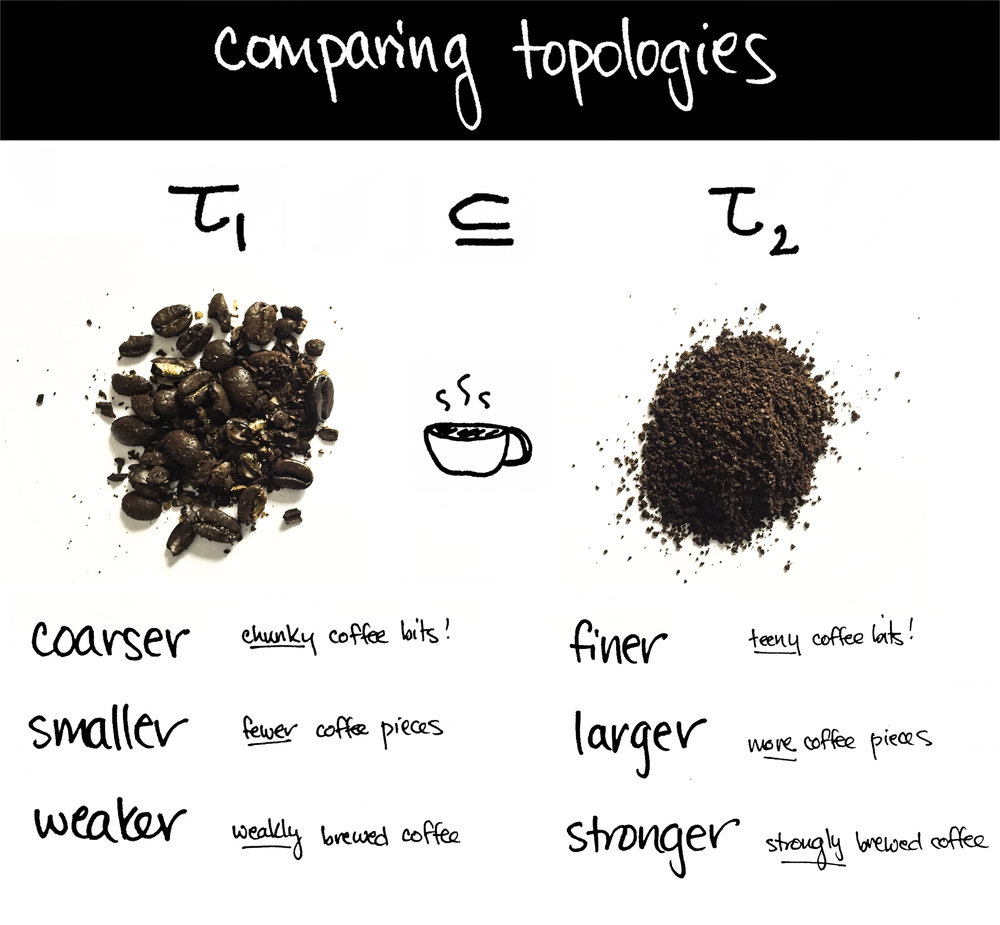
\includegraphics[width=0.65\linewidth]{pics/comparing-topologies-and-coffee.jpg}
    \caption{Comparing topologies and coffee (Credit:
    \href{http://www.math3ma.com/the-back-pocket/2016/8/26/comparing-topologies}{math3ma})}
\end{figure}
For example, assuming we have
\begin{equation}
    f: X\to Y
\end{equation}
where $f$ is any function.

If $X$ has topolgy $\mathcal{T}_X$, we ask then what kind of topolgy on
$Y$ will make $f$ a continuous function. First, all $f^{-1}(V)$, with
$V\in \mathcal{T}_Y$ should be open in $X$. So, the easiest choice is to
make $\mathcal{T}_{Y,\text{min}}=\{\varnothing,Y\}$, this is the
smallest topolgy.  Also, any set $V\in Y$ such that $f^{-1}(V)\notin
\mathcal{T}_X$ should not be in $\mathcal{T}_Y$. Then the largest
topolgy is $\mathcal{T}_{Y,\text{max}}=\{ V\subset Y| f^{-1}(V)\in
\mathcal{T}_X\}$.

If $Y$ has topolgy $\mathcal{T}_Y$, we also ask what kind of topolgy
on $X$ will make $f$ a continuous function. First, all $V\in
\mathcal{T}_Y$, their preimage $f^{-1}(V)$ must be in $\mathcal{T}_X$.
So the smallest topolgy is
$\mathcal{T}_{X,\text{min}}=\{f^{-1}(V)|V\in\mathcal{T}_Y\}$. Than
what about the largest topolgy? We consider, what kind of sets cannot
be inside $\mathcal{T}_X$. First, can $(f^{-1}(V))^c=f^{-1}(V^c)$ be
in $\mathcal{T}_X$? Yes. Since unless the space is connected, there
can be sets being both open and closed (other than $X$ and
$\varnothing$). Any other restrictions? No that I can think of. So,
the largest topolgy $\mathcal{T}_{X,\text{max}}=2^X$, the set of all
subsets of $X$. (The notation \nomen{$2^X$} is taken from the page 4
of book \cite{Singer.Thorpe}.

A summary:
\begin{table}[H]
    \centering
    \caption{Largest and Smallest Topolgies}
    \begin{tabular}{c l l}
        $X\overset{f}{\to}Y$ & Smallest  &Largest \\
        \hline
        Given $\mathcal{T}_X$ & $\mathcal{T}_{Y,\text{min}}=\{\varnothing,Y\}$        & $\mathcal{T}_{Y,\text{max}}=\{ V\subset Y| f^{-1}(V)\in \mathcal{T}_X\}$\\
        Given $\mathcal{T}_Y$ & $\mathcal{T}_{X,\text{min}}=\{f^{-1}(V)|V\in\mathcal{T}_Y\}$ & $\mathcal{T}_{X,\text{max}}=2^X$ \\
        No constraint & $\{\varnothing,X\}$ & $2^X$ \\
        \hline
    \end{tabular}
\end{table}
\paragraph{Facts about subspace/induced topolgy}
Let $Y$ be a subspace of a topological space $X$ wit induced topolgy.
\begin{fact}
    A set $H\subseteq Y$ is open in $Y$ if and only if $H=F\cap Y$
    for some open set $F$ in $X$.
\end{fact}
\begin{fact}
    A set $H\subseteq Y$ is closed in $Y$ if and only if $H=F\cap Y$
    for some closed set $F$ in $X$.
\end{fact}
\begin{fact}
    A set $H$ is open/closed in $X$ $\Rightarrow$ $H$ is open/closed
    in $Y$. But the converse may not be true. The converse statement
    depends on whether $Y$ is open or closed in $X$.
\end{fact}

\subsection{Lebesgue lamme}
\label{sec:Lebesgue lamme}

This is a very important lemma, which is why I gave it a seperate
section. It is labeled (3.11) in book \cite{book}.
\begin{thm}[Lebesgue Lemma]
    \label{lemma:lebesgue-lemma} 
    Let $X$ be a compact metric space and let $\mathscr{F}$ be an open
    cover of $X$. Then there exists a real number $\delta>0$ (called
    the \nomen{Lebesgue number} of $\mathscr{F}$) such that any subset
    of $X$ of diameter less than $\delta$ is contained in some member
    of $\mathscr{F}$.
\end{thm}


\section{A Brief Note of Chapter 4 - Identification Spaces}
\label{sec:Brief-Note-Chapter-4}
\subsection{Identification topology}
\label{sec:Identification topology}

\begin{defi}[Identification Topology]
\nomenclature{Identification Topology}{\nomrefpage.}
Let $X$ be a topological space and let $\mathscr{P}$ be a family of
disjoint nonempty subsets of $X$ such that $\cup \mathscr{P}=X$. Such
a family is usually called a partition of $X$. Let $Y$ be a new space
whose points are the members of $\mathscr{P}$. Let $\pi:X\to Y$ sends
each point of $X$ to the subset of $\mathscr{P}$. Define a topolgy
$\mathcal{T}_Y$ on $Y$ to be the largest topolgy such that the $\pi$
is continuous. This $\mathcal{T}_Y$ is called the idetification topolgy.
And $Y$ is called the \nomen{identification space}.
\end{defi}
\begin{center} \begin{tikzcd}[]
    X\ar[r]\ar[rd] & Y\ar[d,equal] \\
    & \mathscr{P}
\end{tikzcd} \end{center}
\begin{thm}
    Let $Y$ be an idetification space defined as above and let $Z$ be
    an arbitrary topological space. A function $f:Y\to Z$ is
    continuous if and ony if the composition $f\circ \pi:X\to Z$ is
    continuous.
\end{thm}
\begin{center} \begin{tikzcd}[]
    X\ar[r,"\pi"]\ar[rd]\ar[rr,"f\circ\pi",bend left=30] & Y\ar[d,equal]\ar[r,"f"] & Z \\
    & \mathscr{P}
\end{tikzcd} \end{center}
\begin{defi}[Identification Map]
\nomenclature{Identification Map}{\nomrefpage.}
    Let $f:X\to Y$ be an onto continuous map and suppose that the topolgy on $Y$
    is the largest for which $f$ is continuous. Then we call $f$ an
    identification map.
\end{defi}
The naming "identification map" is because:
\begin{thm}
    Any function $f:X\to Y$ gives rise to a partition of $X$ whose
    members are the subsets $\{f^{-1}(y)\}$, where $y\in Y$. Let $Y_*$
    denote the identification space associated with this partition,
    and $\pi:X\to Y_*$ the usual continuous map. 
    $$ \begin{tikzcd}[]
        X\ar[r,"f"]\ar[d,"\pi"] & Y \\
        \{f^{-1}(y)\} \ar[r,equal] & Y_*
    \end{tikzcd} $$
    If $f$ is an identification map, then:
    \begin{enumerate}
        \item the spaces $Y$ and $Y_*$ are homeomorphic;
        \item a function $g:Y\to Z$ is continuous if and only if the
            composition $g\circ f:X\to Z$ is continuous.
    \end{enumerate}
    $$ \begin{tikzcd}[]
        X\ar[r,"f"]\ar[d,"\pi"]\ar[rr,"g\circ f",bend left] 
            & Y\ar[d,equal,"~"]\ar[r,"g"] & Z \\
        \{f^{-1}(y)\} \ar[r,equal] & Y_*
    \end{tikzcd} $$
\end{thm}
\begin{thm}
    Let $f:X\to Y$ be an onto continuous map. If $f$ maps open sets of
    $X$ to open sets of $Y$, or closed sets to closed sets, then $f$
    is an identification map, i.e. $\mathcal{T}_y$ is the largest
    topolgy such that $f$ is continuous.
\end{thm}
\begin{coro}
    \label{coro:idmap-coro}
    Let $f:X\to Y$ be an onto continuous map. If $X$ is compact and
    $Y$ is Hausdorff, then $f$ is an identification map.
\end{coro}

\begin{defi}[Torus]
\nomenclature{Torus}{\nomrefpage.}
Torus is the unit square $[0,1]\times[0,1]$, with 1. opposite edge
identified; 2. four edge points identified.
\end{defi}
\begin{remark}
    The identification map and corollary \ref{coro:idmap-coro} can be
    used to show that torus is homeomorphic to two copies of
    circles:$S^1\times S^1$. This is mentioned in page 68 of
    \cite{book}.
\end{remark}
\begin{defi}[Cone $\textrm{CX}$]
\nomenclature{Cone $\textrm{CX}$}{\nomrefpage.}
    The cone of any space $\textrm{CX}$ is formed from $X\times I$, where
    $I$ is the unit interval $[0,1]$, with certain identification. The
    identification shrinks all points in one surface into one point.  This
    is discussed in page 68 of \cite{book}.
\end{defi}
\begin{figure}[H]
    \centering
    \includegraphics[width=0.5\linewidth]{pics/{Cone-of-a-circle}.pdf}
    \caption{Cone of a Circle (Wikipedia)}
\end{figure}
\begin{remark}
    There is another definition of cone $\textrm{CX}$ when $X$ in imbeded into
    $\mathbb{E}^n$, may be found on page 68 of \cite{book}. Cone
    constructed in this way is called a geometric cone. It is made up
    of all straight line segments that join $v=(0,0,\cdots,1)\in
    \mathbb{E}^{n+1}$ to some point of $X$.
\end{remark}
\begin{lemma}
    The geometric cone on $X$ is homeomorphic to $\textrm{CX}$.
\end{lemma}
\begin{defi}[Quotient Space]
\nomenclature{Quotient Space}{\nomrefpage.}
    Let $X$ be a topological space, $A$ be its subspace. Then $X/A$
    menas the $X$ with subspace $A$ identified to a point.
    \begin{enumerate}
        \item the set $A$.
        \item the individual points of $X\setminus A$.
    \end{enumerate}
\end{defi}
\begin{remark}
    In this notation, $\textrm{CX}$ becomes $(X\times I)/(X\times\{1\})$.
\end{remark}
\begin{fact}
    \begin{equation}
        B^n/S^{n-1} \cong S^n
    \end{equation}
    where $\cong$ menas homeomorphic. This is proved on page 69.
    Intuitively, this is like wrap a lower dimension ball surround the
    higher dimension ball.
\end{fact}

\begin{defi}[$f\cup g$]
\nomenclature{$f\cup g$}{\nomrefpage.}
    Let $X,Y$ $f\cup g$ subsets of a topological space and give each of
    $X,Y$, and$X\cup Y$ the induced topolgy. If $f:X\to Z$ and
    $g:Y\to Z$ are functions which agree on the intersection of $X$
    and $Y$, we can define
    \begin{align}
        f\cup g &: X\cup Y \to Z  \\
        (f\cup g)(x) &= f(x),\, x\in X \nonumber \\
        (f\cup g)(x) &= g(x),\, x\in Y \nonumber
    \end{align}
    We say that $f\cup g$ are formed by 'glueing together' the
    functions $f$ and $g$.
\end{defi}
\begin{lemma}[Glueing lemma (closed)]
    If $X$ and $Y$ are closed in $X\cup Y$, and if both $f$ and $g$
    are continuous, then $f\cup g$ are continuous.
\end{lemma}
Similarly, 
\begin{lemma}[Glueing lemma (open)]
    If $X$ and $Y$ are open in $X\cup Y$, and if both $f$ and $g$
    are continuous, then $f\cup g$ are continuous.
\end{lemma}

These two lemmas are seen as a special case of the following theorem,
explained in page 70.

Define \nomen{$X+Y$} to be the disjoint union of spaces $X,Y$. Define
$j:X+Y \to X\cup Y$ which restrict to either $X$ or $Y$ is just the
inclusion in $X\cup Y$.
\begin{thm}
    If $j$ is an identification map, and if both $f:X\to Z$ and
    $g:X\to Z$ are continuous, then $f\cup g:X\cup Y\to Z$ is
    continuous.
\end{thm}
$$ \begin{tikzcd}[]
    X+Y \ar[r,"j"] & X\cup Y\ar[r,"f\cup g"] & Z \\
    X\ar[rru,"f"] & Y\ar[ru,"g",bend right]
\end{tikzcd}$$

This can be generalized as follows. Let $X_\alpha,\alpha\in A$ be a
family of subsets of a topological space and give each $X_\alpha$ and
the union $\cup X_\alpha$, the induced topolgy. Let $Z$ be a space and
suppose we are given maps $f_\alpha:X_\alpha\to Z$, one for each
$\alpha$ in $A$, such that if $\alpha,\beta\in A$,
$$ 
\eval{f_\alpha}_{X_\alpha\cap X_\beta} = \eval{f_\beta}_{X_\alpha\cap X_\beta}
$$
Define function $F:\cup X_\alpha\to Z$ by glueing together $f_\alpha$.
Let $\oplus X_\alpha$ be the disjoint unin of spaces $X_\alpha$. Let
$j:\oplus X_\alpha \to \cup X_\alpha$ be similarly defined.
\begin{thm}
    If $j$ is an identification map, and if each $f_\alpha$
    is continuous, then $F$ is continuous.
\end{thm}
\textbf{Note}: When $j$ is the identification map, then $\cup
X_\alpha$ has the identification topolgy instead of the subspace
topology. The two will be quite different, as discussed on page 70 to
71 of \cite{book}.

\begin{defi}[Projective space $P^n$]
\nomenclature{Projective space}{\nomrefpage.}
    A discussion of real $P^n$ may be found on page 71.
\end{defi}

\paragraph{\nomen{Attaching maps} and $X\cup_f Y$} Let:
\begin{equation}
    Y \supseteq A \overset{f}{\to} X
\end{equation}
where $X,Y$ are topological spaces, $f$ is continuous. We identify the
disjoint union $X+Y$ using $f$, partitioning them into:
\begin{enumerate}
    \item pairs of points $\{a,f(a)\}$ where $a\in A$;
    \item individual points of $Y\setminus A$;
    \item individual points of $X\setminus \Im(f)$.
\end{enumerate}
The result identification space is denoted $X\cup_f Y$, and $f$ is
called the attaching map. This process can also be viewed as:
\begin{equation}
    X\cup_f Y = (X\amalg Y)/\{f(A)\sim A\}
\end{equation}
\begin{figure}[H]
    \centering
    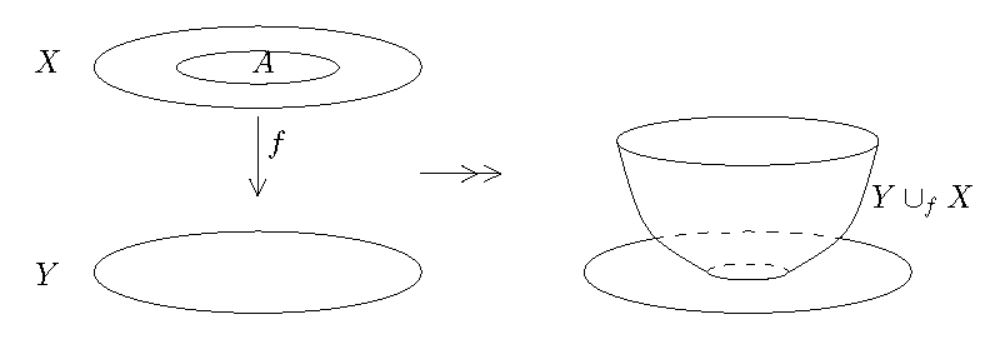
\includegraphics[width=0.6\linewidth]{pics/Attaching-Space.jpg}
    \caption{Attaching Space (credit:
        \href{https://ncatlab.org/nlab/show/Top}{nLab}}
\end{figure}
\begin{ex}
    $P^2$ can be seen as attaching a closed disc $D$ to the boundary
    of $M$, a Mobius strip, as discussed in page 72 of \cite{book}.
    Geometrically, this simply shrinks the boundary of $M$ into a
    point. And an ant travelling around this point can point out the
    direction just as in $P^2$.
\end{ex}
\begin{remark}
    It is remarked that properties such as compactness, connectedness,
    and path-connectedness is inherited in identification. However,
    Hausdorff-ness is not. An counter example can be found in page 72 of
    \cite{book}.
\end{remark}

\subsection{Topological Groups}
\label{sec:Topological-Groups}

In simple words, \nomen{topological groups} are objects that has both
a topolgy on it and a group structure in it. And the two structures
must be compatible. Specifically, the multiplication map $a\cdot b$
and the inverse map $a\to a^{-1}$ are continuous. Homomorphisms
between are both group-homomorphisms and topological-homomorphisms
(continuous maps). Isomorphisms are both group-isomorphisms and
topolgy-isomorphisms (homeomorphisms). A sub-(topological group) is
both a subgroup and has subspace topolgy. For convenience of language,
use \nomen{$\mathcal{TPG}$} denotes the category of topological groups.
\footnote{This notation is nowhere popular or accepted. I use it to
only to save space and time.}
\begin{ex}
    The $\mathbb{R}$ is a topological group. 
    The $\mathbb{Z}$ with discrete topology form the sub-(topological
    group) of $\mathbb{R}$. The quotient $\mathbb{R}/\mathbb{Z}$ forms
    a topological group. The map $f: \mathbb{R}\to S^1$ induces a
    homeomorphism $\mathbb{R}/\mathbb{Z} \cong S^1$, which is also a
    group isomorphisms, i.e. it is a $\mathcal{TPG}$-isomorphism.
\end{ex}
\begin{ex}
    Similarly, $R^n$.
\end{ex}

\begin{ex}
    The circle is also one. The group structure is combination of
    degrees.
\end{ex}
\begin{ex}
    Any group with discrete topology.
\end{ex}
\begin{ex}
    The torus considered as the product of two circles. (Take the
    producttopology and the product group structure.
\end{ex}
\begin{ex}
    Three sphere $S^3$ considered as the unit sphere in the space of
    quaterions $\mathbb{H}$.

    Remember this? :
    $$ \begin{tikzcd}[column sep=small]
        & i\ar[dr] &  \, \\
    k \ar[ur] &
    \ar[u,phantom, "\#"] 
    & j\ar[ll]
    \end{tikzcd} $$
    The unit sphere are unit quaterions, see more
    \href{https://en.wikipedia.org/wiki/Versor}{Versor}.
\end{ex}
\begin{ex}
    The \nomen{orthogonal group} $\mathrm{O}(n)$, of $n\times n$
    orthogonal real matrices. It is easy to check that
    $\mathrm{O}(n-1)$ is a sub-$\mathcal{TPG}$ of $\mathrm{O}(n)$.
\end{ex}

\begin{defi}[Left translation $L_x$]
\nomenclature{Left translation $L_x$}{\nomrefpage.}
    For $x\in G$, the function
    \begin{align}
        L_x: G &\to G \\
          g &\mapsto xg
    \end{align}
    is called a left translation by $x$. Similarly we have
    \nomen{right translation $R_x$}.
\end{defi}
\begin{fact}
    $L_x$ and $R_x$ are homeomorphisms (But not group-isomorphisms).
\end{fact}
\begin{remark}
    This shows that a topological group has a certain homogeneity as a
    topological space. For if $x,y\in G$, then $L_{yx^{-1}}$ maps $x$
    to $y$ and is a homeomorphism. Therefore \textit{$G$ exhibits the
    same topological structure locally near each point}.
\end{remark}
\begin{thm}
    Let $G$ is a topological group, let $K$ be a connected component of $G$
    which contains the identity element. Then $K$ is a closed normal
    subgroup of $G$.
\end{thm}
\begin{fact}
    If $G=\mathrm{O}(n)$, then $K=\mathrm{SO}(n)$.
\end{fact}
\begin{thm}
    In a connected topological group, any neighbourhood of the
    identity element is a set generates the whole group.
\end{thm}
The two theorems above is summarised as

\begin{table}[H]
    \centering
    \caption{caption}
    \begin{tabu}{l c l}
        topology            & $\Rightarrow$ & group/topology \\
        \hline
        $e$ + connected     & $\Rightarrow$ & closed \& normal subgroup \\
        $e$ + neighbourhood & $\Rightarrow$ & generator \\
        \bottomrule
    \end{tabu}
\end{table}

A bit more examples about matrices:
\begin{ex}
    \nomen{$\mathbb{M}(n)$} the $n\times n$ matrices, is not a
    topological group. But its subspace
    \nomen{$\mathrm{GL(n)}$}, specifically,
    $\mathrm{GL(n,\mathbb{R})}$ or $\mathrm{GL(n,\mathbb{C})}$, is a
    topological group. This is demonstrated in page 76, theorem 4.12.
\end{ex}
\begin{fact}
    $\mathrm{GL(n)}$ is not compact. It has two idsjoint nonempty open
    sets: those with positive and those with negative determinants.
\end{fact}
\begin{thm}
    $\mathrm{O}(n)$ and $\mathrm{SO}(n)$ are closed and compact.
    $\mathrm{SO}(n)$ is a sub-$\mathcal{TPG}$ of $\mathrm{O}(n)$.
\end{thm}
\begin{fact}
    $\mathrm{SO}(2)\cong S^1$ and $\mathrm{SO}(3)\cong P^3$.
    Here $\cong$ means isomorphisms of topological groups.
\end{fact}
\begin{remark}
    These two facts established on page 77. The first one can be eaily
    guess. Since a rotation is obviously determined by a rotation
    degree on $S^1$. Mathematically we have
    \begin{equation}
        \left(\begin{array} {cc}
            \cos\theta & -\sin\theta \\
            \sin\theta & \cos\theta 
        \end{array}\right) \cong e^{i\theta}
    \end{equation}

    The second one is proved mathematical in book \cite{book}. But it
    has a physical argument. Remember we have the the homogeneous
    coordinates for $P^3$, such as $[1,\theta_x,\theta_y,\theta_z]$.
    As indicated in my labels, the three free coordinates $\theta_i$
    can be regarded as rotation in 3-dimensional space. This rotation
    preserves the orientation, so it is in $\mathrm{SO}$, not in
    $\mathrm{O}$. 
\end{remark}

\subsection{Orbit Space}
\label{sec:Orbit-Space}
\begin{defi}[Group Action on Topology Space]
\nomenclature{Group Action on Topology Space}{\nomrefpage.}
    A topological group $G$ is said to act as a group of
    homeomorphisms on a space $X$ if each group element (let $g,h\in G$)
    induces a homeomorphism of the space in such a way that:
    \begin{enumerate}
        \item $(hg)(x) = h(g(x)),\, \forall x\in X$;
        \item $e(x)=x,\, \forall x\in X$, where $e=gg^{-1}$;
        \item the function $G\times X\to X$,$(g,x)\mapsto g(x)$ is
            continuous.
    \end{enumerate}
\end{defi}

The subset of $X$, consisting of $g(x)$ for all $g\in G$, is called an
\nomen{orbit} of $x\in X$, written $O(x)$. Thought, it more convenient to
write it just as \nomen{$Gx$}, as in textbooks of abstract algebra.

\begin{fact}
    A common fact in abstract algebra here is: each orbit $Gx$ is
    disjoint. If two $Gx\cap Gy\neq \varnothing$, then $Gx=Gy$.
\end{fact}

By above fact, orbits partitions $X$, hence we can form the
Identification space, with every elements in $X$ identified with their
brothers in the same orbit. The result is \nomen{orbit space $X/G$}.

\begin{ex}
    \label{ex:R-over-Z-T}
    $\mathbb{Z}$ acts on $\mathbb{R}$ by addition $x\mapsto x+n$,
    $x\in \mathbb{R},\,n\in\mathbb{Z}$. It partitioned $\mathbb{R}$
    into intervals, for each $x\in X$, $x\sim x+n,\forall n\in
    \mathbb{Z}$. The orbit space $\mathbb{R}/\mathbb{Z}$ is
    homeomorphic to $S^1$.
\end{ex}

An action $G$ on $X$ is called \nomen{transitive}, if and only if the
orbit space $X/G$ is the trivial point $\{1\}$. Or equivalently, the
only orbit is the whole space, i.e. $Gx=G,\,\forall x\in G$.

\begin{ex}
    The orthogonal action $O(n)$ on $S^{n-1}$ is transitive.
    Physically, this is saying that $\forall x\in S^{n-1}$, it can be
    rotated into $\forall y\in S^{n-1}$. A mathematical proof is on
    page 79 of \cite{book}
\end{ex}

\paragraph{A lot of examples from book \cite{book}}$ $

\begin{ex}
    Extending example \ref{ex:R-over-Z-T}:
\begin{equation}
    \mathbb{E}^2/(\mathbb{Z}\times\mathbb{Z}) = T\text{ (torus)}
\end{equation}
    Here $=$ means homeomorphism.
\end{ex}
\begin{ex}
    \begin{equation}
        S^n/\mathbb{Z}_2 = P^n
    \end{equation}
    Here $=$ means homeomorphism.
\end{ex}
\begin{ex}[Three ways of $\mathbb{Z}_2$ acting on $T$]
    The detailed procedure is to be found on page 91 of \cite{book}.
    Here's a picture to visualize the action:
    \begin{figure}[H]
        \centering
        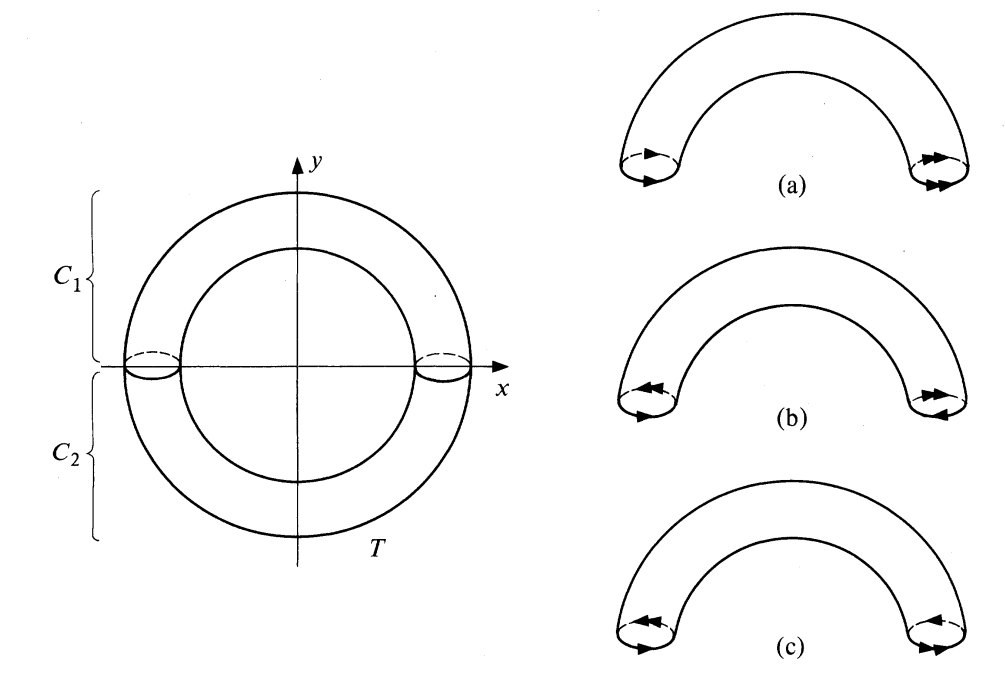
\includegraphics[width=0.8\linewidth]{pics/3-ways-Z2-on-T.PNG}
        \caption{$ $}
    \end{figure}
    The results are (a) a sphere; (b) a torus; (c) a Klein bottle.
\end{ex}
\begin{ex}
    If $G$ is a topological group, and $H$ is
    $\mathcal{TPG}$-subgroup. Then, the left cosets of right cosets
    can be canonically seen as orbits. See more on page 81, example 4.
\end{ex}
\begin{ex}
\begin{align}
    \mathrm{O}(n)/\mathrm{O}(n-1) &= S^{n-1} \\
    \mathrm{SO}(n)/\mathrm{SO}(n-1) &= S^{n-1}
\end{align}
    Here $=$ means homeomorphism. The first is established
    mathematically in page 82 of \cite{book}. The second is mentioned
    there, indicating a similar proof.

    Here I give an argument. Consider a unit vector $y$ in $S^{n-1}$, if
    we want to rotate another unit vector $e_1$ to $y$, since the
    action is transitive, we can easily find a $A\in \mathrm{O}(n)$ to
    do this. But in addition, we can also find that $A\cdot B$, where
    $B\in \mathrm{O}(n-1)$ rotates the space around $e_1$ (thus
    leaving $e_1$ un-affected) also do our job. So there is an
    $\mathrm{O}(n-1)$ redundancy in $\mathrm{O}(n)\to S^{n-1}$.
    Similar for the second relation.
\end{ex}

\begin{thm}
    Let $G$ acts on $X$ and suppose that both $G$ and $X/G$ are
    connected, then $X$ is connected.
\end{thm}
\begin{fact}
    Using the theorem above, one can deduce that: $\mathrm{SO}(1)$ is
    connected, $S^{n-1}$ is connected, so $\mathrm{SO}(n)$ is
    connected.
\end{fact}

Next, the book \cite{book} (page 82 to 85) introduces several three
spaces (\nomen{Lens space}, \nomen{irrational flow} on $T$ torus,
\nomen{fundamental region} or in my word \textit{space filling
shapes}) and two group \nomen{Euclidean group} (page 84) and
\nomen{plane-crystallographic group} (page 85). To save time, I leave
here only some pictures:
\begin{figure}[H]
    \centering
    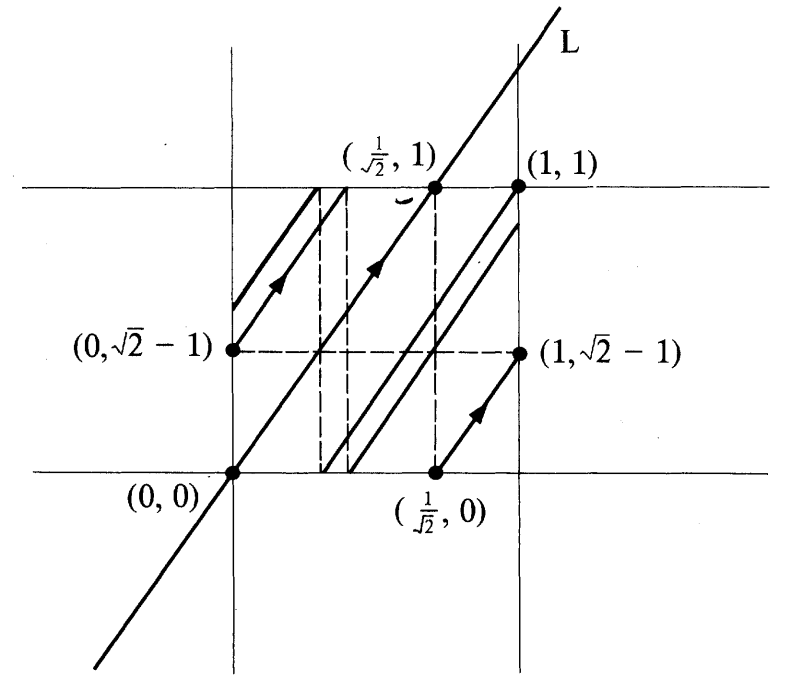
\includegraphics[width=0.8\linewidth]{pics/irrational-flow.png}
    \caption{Irrational Flow on $T$}
\end{figure}
\begin{figure}[H]
    \centering
    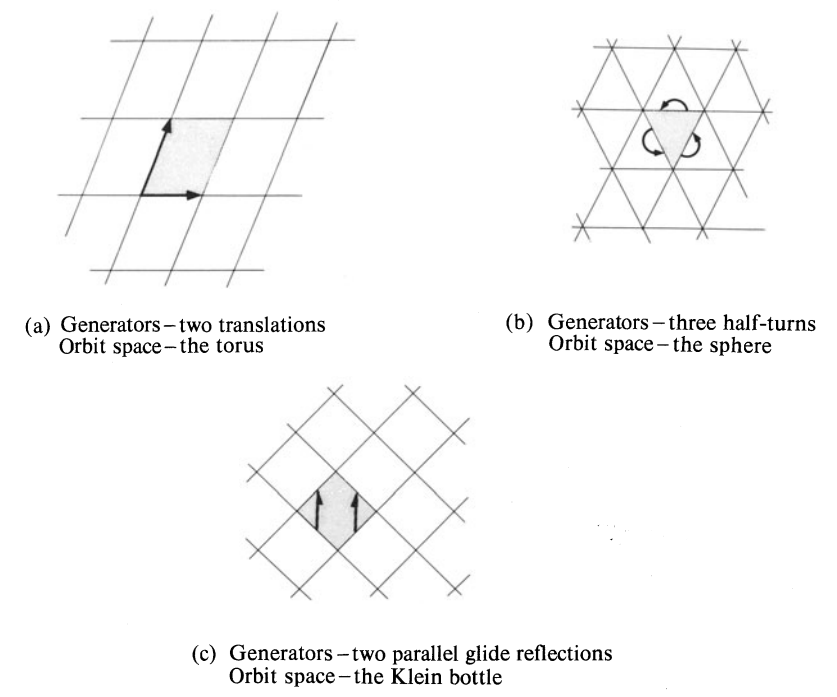
\includegraphics[width=0.8\linewidth]{pics/space-filling-shapes.png}
    \caption{Space-filling Shapes}
\end{figure}




\section{Chapter 5 - Fundamental Groups}
\label{sec:Chapter-5-Fundamental-Groups}

\subsection{Homotopic maps}
\label{sec:Homotopic-maps}

By a \nomen{loop} we mena a continuous map $\alpha:I\to X$ such that
$\alpha(0)=\alpha(1)$. We can view is also as a continuous map
$\alpha:S^1 \to X$. It is said to be based at the point
$\alpha(0)$. Two loops $\alpha$ and $\beta$ with the same \nomen{base
point} can be multiplied, and their product is defined on page 87.
A visualization is here:
% cd 1 todo

But this product is not sufficient to become a group. At least, the
multiplication is not associative:
% cd 2 todo

But clearly the two result are exactly if we do care how long they
occupy on the interval $I$, if the interval $I$ is considered as a
time parameter. So we define the following homotopy relation between
loops. If we can find a family $\{f_r\}$ of maps, one for each $r\in
[0,1]$, such that $f_0=\alpha$, $f_1=\beta$, then we say that the
loops $\alpha$ and $\beta$ are homotopic. Schematically,
% cd 3 todo

This relation can be generalized to any continuous maps:
\begin{defi}[Homotopic]
\nomenclature{Homotopic}{\nomrefpage.}
    Let $f,g: X \to Y$ be continuous maps. Then $f$ is homotopic to
    $g$ if there exists a map $F:X \times I\to Y$ such that $F(x,O) =
    f(x)$ and $F(x,1) = g(x)$ for alt points $x\in X$.
\end{defi}

The map $F$ is called a \nomen{homotopy} from $f$ to $g$, and we write
\nomen{$f\simeq_F g$}. In addition, if $f$ and $g$ agree on some
$A\subset X$, we may wish to deform $f$ to $g$ without altering the
values of $f$ on $A$. In this case we ask for a homotopy $F$ from $f$
to $g$ with the additional property that 
\begin{equation}
    F(a,t)=f(a) \text{ for all $a\in A$, for all $t\in I$}
\end{equation}
when such a homotopy exists, we say the \nomen{$f$ is homotopic to $g$
relative to $A$} and write \nomen{$f\simeq_F g$ rel $A$}.
% cd 4 todo


When $f$ and $g$ are loops, then the homotopic relation for loops are
just saying that $f\simeq g$ rel $\{0,1\}$.

% fig 5.1 p 88 todo

\begin{ex}
    The author shows on page 88 of \cite{book} that: when $C$ is a
    convex subset of a euclidean space, let $f,g:X\to C$ be continuous
    maps, then $f\simeq_F g$, where $F$ is $F(x,t)=(1-t)f(x)+tg(x)$.
    Note that if $f$ and $g$ agree on a subset $A$ of $X$, then this
    homotopy is a homotopy relative to $A$. This $F$ is called a
    \nomen{straight-line homotopy}.
\end{ex}
\begin{ex}
    Let $f,g:X\to S^n$ be continuous maps. We can take $S^n$ to be the
    unit sphere in $\mathbb{E}^{n+1}$, and think of $f,g$ as
    continuous maps into $\mathbb{E}^{n+1}$, then we may form a
    straight-line homotopy from $f$ to $g$ by:
    \begin{equation}
        F(x,t) = \frac{(1-t)f(x)+tg(x)}{||(1-t)f(x)+tg(x)||}
    \end{equation}
    But why we are  % yes why! TODO
\end{ex}
\begin{ex}
    This is example is best illustrated by pictures:
    % fig 5.2 todo
    Geometrieally, $\alpha$ winds eaeh of the segments
    $[O,\frac{1}{2}]$, $[\frac{1}{2},\frac{3}{4}]$, $[\frac{3}{4}, 1]$
    once round the eirc1e, the first two being wound in an
    anticlockwise direetion, and the third clockwise. The loop $\beta$
    simply winds the whole interval $[0,1]$ once round the circle
    anticlockwise.

    The book\cite{book} gives a homotopy $F$ between $\alpha$ and
    $\beta$ on page 89. But it is best to imagine $\alpha$ and $\beta$
    being metal coils, and this $F$ just describes the process when
    one magically strach and unfold the coil from $\alpha$ to $\beta$.

    Notice that this coil is connected head to tail, so it is
    essential that there is not pole inside the coil in order that one
    can unfold the coil from $\alpha$ to $\beta$.
\end{ex}

I think we already feel this, but the book proves it on page 90, that

\begin{lemma}
    The relation of 'homotopy' is an equivalence relation on the set
    of all maps from $X$ to $Y$.
\end{lemma}

Also
\begin{lemma}
    The relation of 'homotopy relative to a subset $A$ of $X$' is an
    equivalence relation on the set of all maps from $X$ to $Y$ which
    agree with some give map on $A$.
\end{lemma}

The book also mentions that
\begin{lemma}
    Homotopy behaves well with respect to composition of maps
\end{lemma}
which means precisely that:
\begin{itemize}
    \item If $f\simeq_F g$ rel $A$, then $hf\simeq_{hF} hg$ rel $A$.
        $$ \begin{tikzcd}[]
            A\subset X \ar[r,"f",bend left]\ar[r,"g",bend right]
                & Y \ar[r,"h"] & Z
        \end{tikzcd}$$
    \item If $g\simeq_G h$ rel $B$, then $gf\simeq_F hf$ rel $f^{-1}B$
        via the homotopy $F(x,t)=G(f(x),t)$.
        $$ \begin{tikzcd}[]
            X\ar[r,"f"] & Y \ar[r,"g",bend left]\ar[r,"h",bend right]
             & Z \\
            f^{-1}B\ar[u,phantom,"\subset"
            {anchor=south,rotate=90,left=0,near end}]
                &
            B\ar[u,phantom,"\subset" {anchor=south,rotate=90,left=0,near
            end}] & \, 
        \end{tikzcd}$$
\end{itemize}

\subsection{Construction of the fundamental group}
\label{sec:Construction-of-the-fundamental-group}

\begin{thm}
    The set of homotopy classes of loops in $X$ based at $p\in X$
    forms a group under the multiplication
    $\braket{\alpha}\cdot\braket{\beta}=\braket{\alpha\cdot\beta}$.
    The identity and inverse elements are defined on page 92 and 93 of
    \cite{book}.
\end{thm}
\begin{remark}
    Notice that the fundamental group dependes heavily on the base
    point. Especially when the space $X$ is disconnected. A natural
    intuition is that when the space is path-connected, then any two
    paths can be connected. If two points can be connected, then two
    loops based on different points can be connected. That why we have
    the following.
\end{remark}
\begin{thm}
    If $X$ is a path-connected then $\pi_1(X,p)$ $\pi_1(X,q)$ are
    isomorphic for any two points $p,q\in X$.
\end{thm}
\begin{proof}
    The proof is on page 94 of \cite{book}.
\end{proof}
\begin{defi}[$f_*$]
\nomenclature{$f_*$}{\nomrefpage.}
Suppose we have a continuous map $f:X\to Y$, $f$ can induce a map
($p\in X,q\in Y$ and $q=f(p)$).
    \begin{align}
        f_* : \pi_1(X,p) &\to \pi_1(Y,q) \\
        \braket{\alpha} &\mapsto \braket{f\circ \alpha}
    \end{align}
This map is actually a homomorphism.
\end{defi}
\begin{fact}
By construction, we have for
$$ \begin{tikzcd}[]
    X\ar[r,"f"] & Y\ar[r,"g"] & Z
\end{tikzcd}$$
\begin{align}
    (g\circ f)_* = g_* \circ f_*
\end{align}
\end{fact}
\begin{fact}
With a homeomorphism $h:X\to Y$ and the above fact, we see that
homeomorphic spaces have isomorphic fundamental groups.
\end{fact}
\subsection{Sectin 5.3}
\label{sec:Sectin-5.3}
This section calculates the following facts:
\begin{table}[H]
    \centering
    \begin{tabular}{c c c}
        \hline
        \#&  Space                           & Fundamental group \\
          \hline
        1 &  Conves subset of $\mathbb{E}^n$ & \{e\} \\
        2 &  Circle                          & $\mathbb{Z}$ \\
        3 & $S^1$                           & $\mathbb{Z}$ \\
        4 & $S^n,\, n\geq 2$                & \{e\} \\
        5 & Torus $S^1\times S^1$           & $\Z\times\Z$ \\
        6 & $P^n,, n\geq 2$                 & $\Z_2$ \\
        7 & Klein bottle                    & $\{a,b|a^2=b^2\}$ \\
        8 & Len space $L(p,q)$              & $\Z_p$ \\
          \hline
    \end{tabular}
\end{table}

\paragraph{Convex subset of $\E^n$} is on page 96 of \cite{book}.
\begin{defi}[simply connected]
\nomenclature{simply connected}{\nomrefpage.}
    A path-connected space whose fundamental group is trivial is said
    to be simply connected.
\end{defi}

\paragraph{The $n$-sphere $S^n$} is on page 99. To prove it, we
require a theorem:
\begin{thm}
    Let $X$ be a space which can be written as the union of two simply
    connected open sets $U,V$ in such a way that $U\cap V$ is
    path-connected. Then $X$ is simply connected.
\end{thm}
\begin{proof}
    Proof is on page 99 of \cite{book}. It requires the Lebesgue lemma
    \ref{thm:lebesgue-lemma}. A picture illustrating the proof is
    provided here:
    \begin{figure}[H]
        \centering
        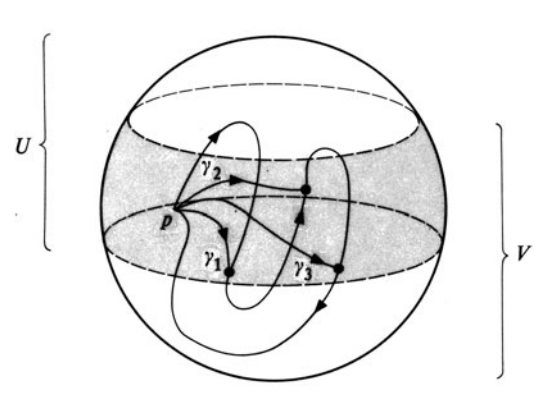
\includegraphics[width=0.6\linewidth]
        {pics/n-sphere-is-simply-con.PNG}
    \end{figure}
\end{proof}
Then, the two cover of $S^n$ are simply $U=S^n-\{x\}$ and
$V=S^n-\{y\}$, where $x,y$ are two distinct points on $S^n$. Since $U$
and $V$ are homeomorphic to $\E^n$, $S^n$ is simply-connected.

\subsection{Continued Section 5.3}
\label{sec:Continued-Section-5.3}
In this section, I will follow the lecture by professor Li Qin.
We show that
\begin{thm}
    $$\pi_1 (S^1) = \mathbb{Z} $$
\end{thm}

\begin{proof}
    Given any integer $n\in \mathbb{Z}$, we give a loop by associatng
    each $n$ 
    \begin{align*}
        \pi : \mathbb{R} \to S^1 \\
        t \mapsto e^{2\pi it}
    \end{align*}
    Define 
    \begin{align}
        \gamma_n : [0,1] \to \mathbb{R} \\
        s\mapsto n s
    \end{align}
    Then $\phi_n:= \pi\circ \gamma_n$ has the property that
    $\phi_n(0)=1$, $\phi_n(1)=1$. So we obtain 
    \begin{equation}
        \phi: \mathbb{Z} \to \pi_1  (S^1)
    \end{equation}
    Geometrically, we $\phi_n$ loops around $S^1$ in $n$ turns.

    We need to prove that $\phi$ is a isomorphism. This is done by:
    \begin{enumerate}
        \item Prove that $\phi$ is a homomorphism;
        \item Prove that $\phi$ is bijective.
    \end{enumerate}
    First,
    \begin{align*}
        \gamma_n: s \mapsto n s \\
        \gamma_m: s\mapsto m s\\
    \end{align*}
    We need
    \begin{align*}
        \braket{\pi\circ \gamma_{m+n}} =
        \braket{\pi\circ\gamma_m}\braket{\pi\circ \gamma_n}\\
    \end{align*}
    Define $\sigma:[0,1]\to \mathbb{R}$, $s\mapsto \gamma_n(s)+m$,
    this is a translation of real line. Then $\pi\circ \sigma =
    \pi\circ \gamma_n$. Then
    \begin{align*}
        \braket{\pi\circ\gamma_m}\braket{\pi\circ \gamma_n}
        = \braket{\pi\circ\gamma_m} \braket{\pi\circ\sigma}
        = \braket{\pi\circ(\gamma_m\circ \sigma)}
    \end{align*}
    $\gamma_{m+n}$ has the same domain and codomain of $\gamma_m \circ
    \sigma$, and they obviously share the same start and the same end
    point. Therefore these two path are homotopic relative to
    $\{0,1\}$.
    Therefore
    \begin{equation}
        \braket{\pi\circ \gamma_{m+n}} =
        \braket{\pi\circ(\gamma_m\circ\sigma)}
    \end{equation}
    Or
    \begin{equation}
        \phi_{m+n} = \phi_{m}\phi_n
    \end{equation}

    Second, we need to show that this map is surjective. Notice that
    $\pi:\mathbb{R}\to S^1$, $t\mapsto e^{2\pi i t}$, is like a
    projection of a circulatory path onto a circle $S^1$. This map is
    locally homeomorphic. We can find a cover of $S^1$ as the
    combination of
    \begin{align*}
        U = S^1\setminus \{-1\} \\
        V = S^1\setminus \{1\}
    \end{align*}
    Then $\pi^{-1}(V)$ are the intervals on $\mathbb{R}$ excluding the
    whole integer points. Similarly, $\pi^{-1}(U)$ are those intervals
    on $\mathbb{R}$ excluding those half-integer points. In each of those
    intervals the map $\pi$ is bijective.
    Now we need a lemma:
    \begin{lemma}[Path-lifting lemma]
        \label{thm:path-lifting-lemma-1}
        \begin{equation}
            \begin{tikzcd}[]
                \, & \mathbb{R}\ar[d,"\pi"] \\
                {[0,1]}\ar[r,"\sigma"]\ar[ru,"f"] & S^1
            \end{tikzcd}
        \end{equation}
        Assuming we have $\pi$ and $\sigma$, both are continuous maps.
        More specifically, $\sigma$ is a path in $S^1$ which begins at the
        point $1\in S^1$. Then there is a unique path $\tilde\sigma$ in
        $\mathbb{R}$ which begins at $0\in \R$ and satisfies $\pi\circ
        \tilde\sigma = \sigma$.
    \end{lemma}
    \begin{proof}
        The proof is on page 97 to 98 of \cite{book}. The class gives
        me enough intuition to understand the proof.

        The intuition is that, by Lebesgue lemma, we can divide the
        interval $[0,1]$ fine enough such that each divided part  is
        maped to only one of the cover $U$ or $V$.  We thus break a
        path $\sigma$ into small paths $\sigma_i$. Each $\sigma_i$ can
        be lifted into a path $\tilde\sigma_i$ in $\R$. But such
        lifting can be arbitrary because the inverse of $\pi$ is not a
        good function. To resolve this ambiguity, one requires the
        first path should starts with $0\in\R$, and the second should
        be continuously connected to the first, and so is the third,
        fourth, etc. This fixes the ambiguity and the paths
        $\tilde\sigma_i$ when connected give the required path
        $\tilde\sigma$.
    \end{proof}
    Note that $\tilde\sigma(0)=0$, $\tilde\sigma(1)$ is an integer.
    Now for any loop $\gamma:[0,1]\to S^1$ based at $1$, we can find a
    lifting $\tilde\gamma:[0,1]\to \mathbb{R}$ such that
    $\tilde\gamma(0)=0$,$\tilde\gamma(1)=n$, and $\gamma = \pi\circ
    \tilde\gamma$. Then $\tilde\gamma \cong \gamma_n$ rel $\{0,1\}$,
    also $\braket{\pi\circ\tilde\gamma}=\braket{\pi\circ\gamma_n}$.
    Hence for any path $\gamma$ we find a $n$ such that
    $\gamma=\phi(n)$. So \textit{the map is surjective}.



    We need another lemma to prove that it is injective.
    \begin{lemma}[Homotopy-lifting lemma]
        If $F:[0,1]\times[0,1]\to S^1$ is a map such that
        $F(0,t)=F(1,t)=1$ for $0\leq t\leq 1$, then there exists a
        unique $\widetilde F: [0,1]\times[0,1]\to \mathbb{R}$ such that
        \begin{align}
            \pi\circ \widetilde F = F \\
            \widetilde F(0,t) =0,\, 0\leq t\leq 1
        \end{align}
    \end{lemma}
    % TODO Graph here. DC 1
    \begin{proof}
        The proof is on page 98 of \cite{book}. The idea is exactly
        the same as in lemma~\ref{thm:path-lifting-lemma-1}.
    \end{proof}
    Now we proof that the map $\phi$ is injective. Suffice to prove
    that $\Ker(\phi)$ is trivial. Suppose $\phi(n)=\pi\circ \gamma_n$
    is homotopic to the constant loop. Then choose a homotopy $F$
    from $\pi\circ\gamma_n$ to the constant loop. By the
    homotopy-lifting lemma we can find $\widetilde F: [0,1]\times[0,1]\to
    \mathbb{R}$ such that $\pi\circ \widetilde F = F$. Also
    $\widetilde F(0,t)=0$.
    We can find the vertical bottom is $0$ and verticl top is
    $\gamma_n$. Right line is integers and can only be $0$ Hence
    $\gamma_n$ starts at $0$ and ends at $0$.
    One can find that $\gamma_n\cong 0$. This completes the proof of
    injectivity. Hence completes the whole proof.
\end{proof}

We have an application,
\begin{thm}[Brouwer Fixed Point theorem] % TODO brower? broer?
    A contiuous map $f:B^2\to B^2$ ($B^2:2D$-closed dicks) must have a
fixed point. That is, $\exists x\in B^2$ such that $f(x)=x$.
\end{thm}
\begin{proof}
    Assuming that this theorem is false, that is $\forall x\in B^2$,
    $x\neq f(x)$, then we have a straight path from $f(x)$ to $x$. We can
    extends this path to cuts the boundary of $B^2$ at $h(x)$. This is
    for all $x\in B^2$, hence we have a map $h: B^2 \to S^1$. Also,
    $h|_{S^1}$ is obvious an identity map. But $S^1$ can be included
    inside $B^2$, so we have:
    \begin{equation}
        S^1 \to B^2 \to S^1 % TODO add function labels
    \end{equation}
    Hence we have a series of homomorphism of fundamental groups:
    \begin{equation}
        \pi_1 (S^1) \to \pi_1 (B^2) \to \pi_1(S^1)
    \end{equation}
    and the composite is identity map. But observe that $B^2$ is a
    convex set and hence its fundamental group is trivial. But $S^1$
    has non-trivial fundamental group.
\end{proof}
\begin{remark}
    This theorem can be extended to higher dimensional case. But the
    proof cannot be the same because for higher dimension $\pi_1(S^n)$
    is no longer non-trivial.
\end{remark}

Another application, which we need a theorem to help:
\begin{thm}
    \begin{equation}
        \pi_1 (X\times Y, (x_0,y_0)) = \pi_1 (X,x_0) \otimes \pi_1
        (X,y_0)
    \end{equation}
\end{thm}
\begin{proof}
    We use the projection maps: $P_1$ and $P_2$.
    Then, the map
    \begin{align*}
        (P_1)_*: \pi_1 (X\times Y) \to \pi_1(X) \\
        (P_2)_*: \pi_1 (X\times Y) \to \pi_1(Y)
    \end{align*}
    and their composition formed into
    \begin{align*}
        \braket{\alpha}\mapsto
        (\braket{P_1\circ\alpha},\braket{P_2\circ\alpha})
    \end{align*}
    this map is surjective, injective, and is homomorphism.
    The detail can be found on page page 101 of \cite{book}.
\end{proof}

\begin{fact}
By this theorem, the two objects $S^2$ and $S^1\times S^1$ is not
homeomorphic, since their fundamental groups are not the same (the
former is trivial and the later is $\mathbb{Z}\times\mathbb{Z}$).
\end{fact}

% TODO homework: pro 13 of page 95.

\subsection{Homotopy Type}
\label{sec:Homotopy-Type}

Notice that a homeomorphic map will make two space have the same
fundamental group, but two space having the same fundamental group may
not be homeomorphic. For example, the plane and the $S^2$ both have
the same $\pi_1=\{e\}$, but the plane is not compact while the
$2$-sphere is, i.e. they are not homeomorphic.

Notice also that homeomorphic requires $fg^{-1}=\id$, whereas under
homotopic relation, we may require $fg^{-1}\cong\id$. Therefore we may
also define a new type of relationship between topological spaces:

\begin{defi}[Homotopy type]
\nomenclature{Homotopy type}{\nomrefpage.}
    Two spaces $X$ and $Y$ have the same homotopy type, or they are
    homotopy equivalent, if there exist maps:
    $$ \begin{tikzcd}[]
        X\ar[r,"f",bend left] & Y\ar[l,"g",bend left]
    \end{tikzcd}$$
    such that $g\circ f\cong \id_X$, and $f\circ g\cong\id_Y$.
\end{defi}
\begin{fact}
This relationship must be an equivalence relation on topological
spaces, as confirmed by lemma (5.16) on page 103 of \cite{book}.
\end{fact}

\begin{defi}[Deformation retraction]
\nomenclature{Deformation retraction}{\nomrefpage.}
    Let $A$ be a subspace of $X$. Let a homotopy $G:X\times I\to X$ which
    is relative to $A$ and for which
    $$ \begin{cases}
        G(x,0)=x & \\
        G(x,1)\in A
    \end{cases}$$
    for all $x\in X$. Then $G$ will be called a deformation retraction
    of $X$ onto $A$.
\end{defi}
\begin{remark}
    If there is a deformation retraction of $X$ onto $A$, then of
    course $X$ and $A$ have the same homotopy type.
\end{remark}
Following is an example of a deformation retraction:
\begin{figure}[H]
    \centering
    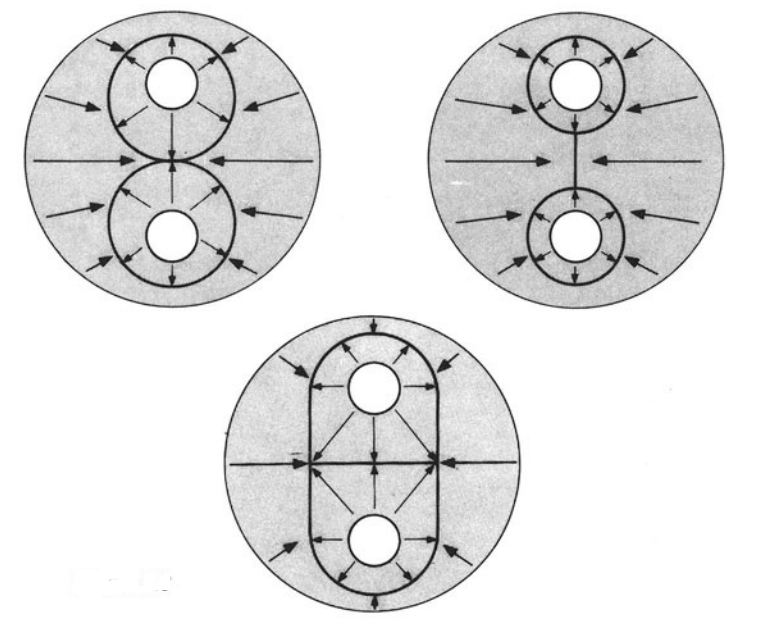
\includegraphics[width=0.8\linewidth]{pics/deformation-retraction.PNG}
    \caption{Three Deformation Retractions (from \cite{book})}
\end{figure}

Exmaples from the book:
\begin{ex}
    Homeomorphic spaces have the same homotopy type.
\end{ex}
\begin{ex}
    Any convex subset of a euclidean space is homotopy equivalent to a
    point.
\end{ex}
\begin{ex}
    $\E^n\setminus \{0\}$ has the homotopy type of $S^{n-1}$. This is
    shown on page 104 of \cite{book}, and is illustrated there by:
    \begin{figure}[H]
        \centering
        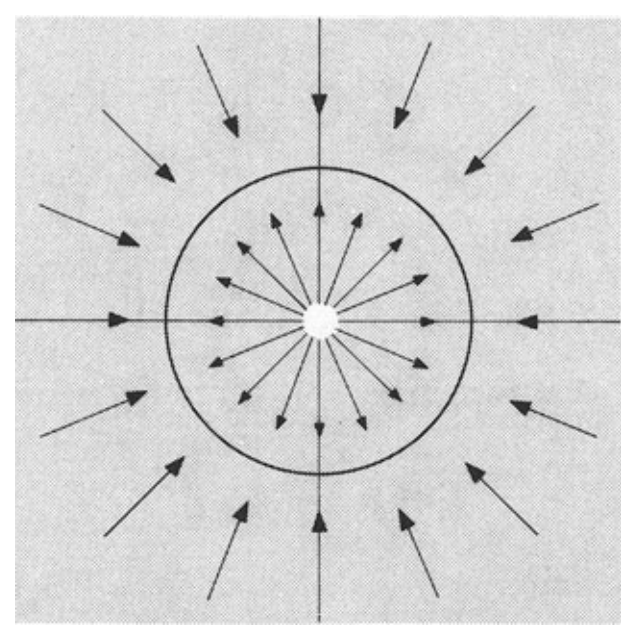
\includegraphics[width=0.6\linewidth]{pics/En-0-and-S-n-1.PNG}
        \caption{$E^n\setminus\{0\}$ and $S^{n-1}$}
    \end{figure}
\end{ex}

\begin{thm}
    If $f\cong_F g:X\to Y$ then $g_*:\pi_1(X,p)\to \pi_1(Y,g(p))$ is
    equal to the composition
    \begin{equation} \begin{tikzcd}[]
        \pi_1(X,p)\ar[r,"f_*"]&\pi_1(Y,f(p))\ar[r,"\gamma_*"]
            &\pi_1(Y,g(p))
    \end{tikzcd} \end{equation}
    where $\gamma$ is the path joining $f(p)$ to $g(p)$ in $Y$ defined
    by $\gamma(s)=F(p,s)$.
\end{thm}
\begin{proof}
    Proof can be found on page 105 of \cite{book}.
\end{proof}

\begin{thm}
    If two path-connected spaces are of the same homotopy type, then
    they have isomorphic fundamental group.
\end{thm}
\begin{proof}
    Proof can be found on page 106 of \cite{book}. Here's a note using
    the notation in that book:
    $$ \begin{tikzcd}[]
        X\ar[r,"f",bend left] & Y\ar[l,"g",bend left]
    \end{tikzcd}$$
    It should be noticed that the continuity allows one to identify the
    diagram:
    $$ \begin{tikzcd}[]
        \pi_1(X,p)\ar[r,"(gf)_*"]\ar[rr,"\id",bend right]
            &\pi_1(X,gf(p))\ar[r,"\gamma^{-1}_*"]
            &\pi_1(X,p)
    \end{tikzcd} $$
    with the diagram:
    $$ \begin{tikzcd}[]
        \pi_1(X)\ar[r,"(gf)_*"]\ar[rr,"\id",bend right]
            &\pi_1(X)\ar[r,"\gamma^{-1}_*"]
            &\pi_1(X)
    \end{tikzcd} $$
\end{proof}

\begin{fact}
Using above fact, we can find that the M\"obius strip, the cylinder,
the punctured plane $\E^2\setminus\{0\}$, and the solid torus, all
have the homotopy type of a circle $S^1$, and consequiently have $\Z$
as fundamental group.
\end{fact}
\begin{fact}
    Also, $\E^n\setminus\{0\}$ deformation-retracts onto $S^{n-1}$ and
    is therefore a simply connected space when $n\geq 3$.
\end{fact}

\begin{defi}[Contractible]
\nomenclature{Contractible}{\nomrefpage.}
    A space $X$ is called contractible if the identity map $\id_X$ is
    homotopic to the constant map at some point of $X$.
\end{defi}
\begin{thm}$ $

    \begin{enumerate}
        \item A space is contractible if and only if it has the
            homotopy type of a point.
        \item A contractible space is simply connected.
        \item Any two maps into a contractible space are homotopic.
        \item If $X$ is contractible, then $\id_X$ is homotopic to the
            constant map at $x$ for any $x\in X$.
    \end{enumerate}
\end{thm}
\begin{ex}
    Here is a contractible space that is really hard to imagin. It is
    called the topologist's dunce hat. It is formed by identifying the
    sides of a triangle in the manner indicated in the following
    figure:
    \begin{figure}[H]
        \centering
        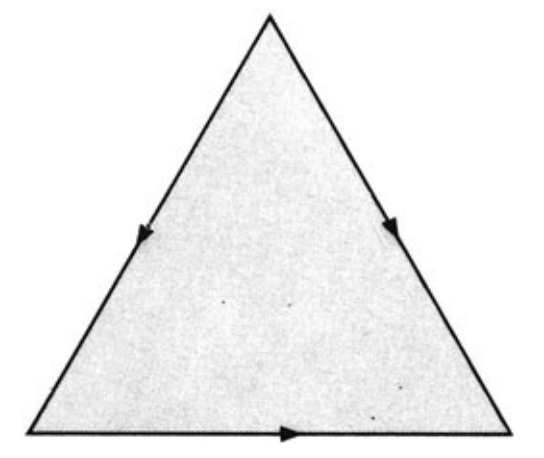
\includegraphics[width=0.4\linewidth]{pics/topo-dunce-hat.PNG}
        \caption{Topologist's dunce hat}
        \label{fig:topo-d-hat}
    \end{figure}
    You may imagin identify a pair of sides, then identify the
    identitied edge to the resting side. The direction for identifying
    is really important.
    This space is contractible. Despite some hard words said by the
    book, it is really simple to see on figure~\ref{fig:topo-d-hat}.
    Draw any loop on it and shrink it. Noticing that all edges are
    identified, though in some odd direction.
\end{ex}



\textbf{Note:} The teacher decided to temporarily switched to the next
chapter, which is about a technique to patch the whole space. He will
come back to the remaining sections of chapter 5 later.

\section{Chapter 6 - Triangulation}
\label{sec:Chapter6-Triangulation}
\subsection{Section 6.1 Triangulating Spaces}
\label{sec:Triangulating-Spaces}

He gave to examples first,
\begin{ex}
    A trivial example:
    \begin{figure}[H]
        \centering
        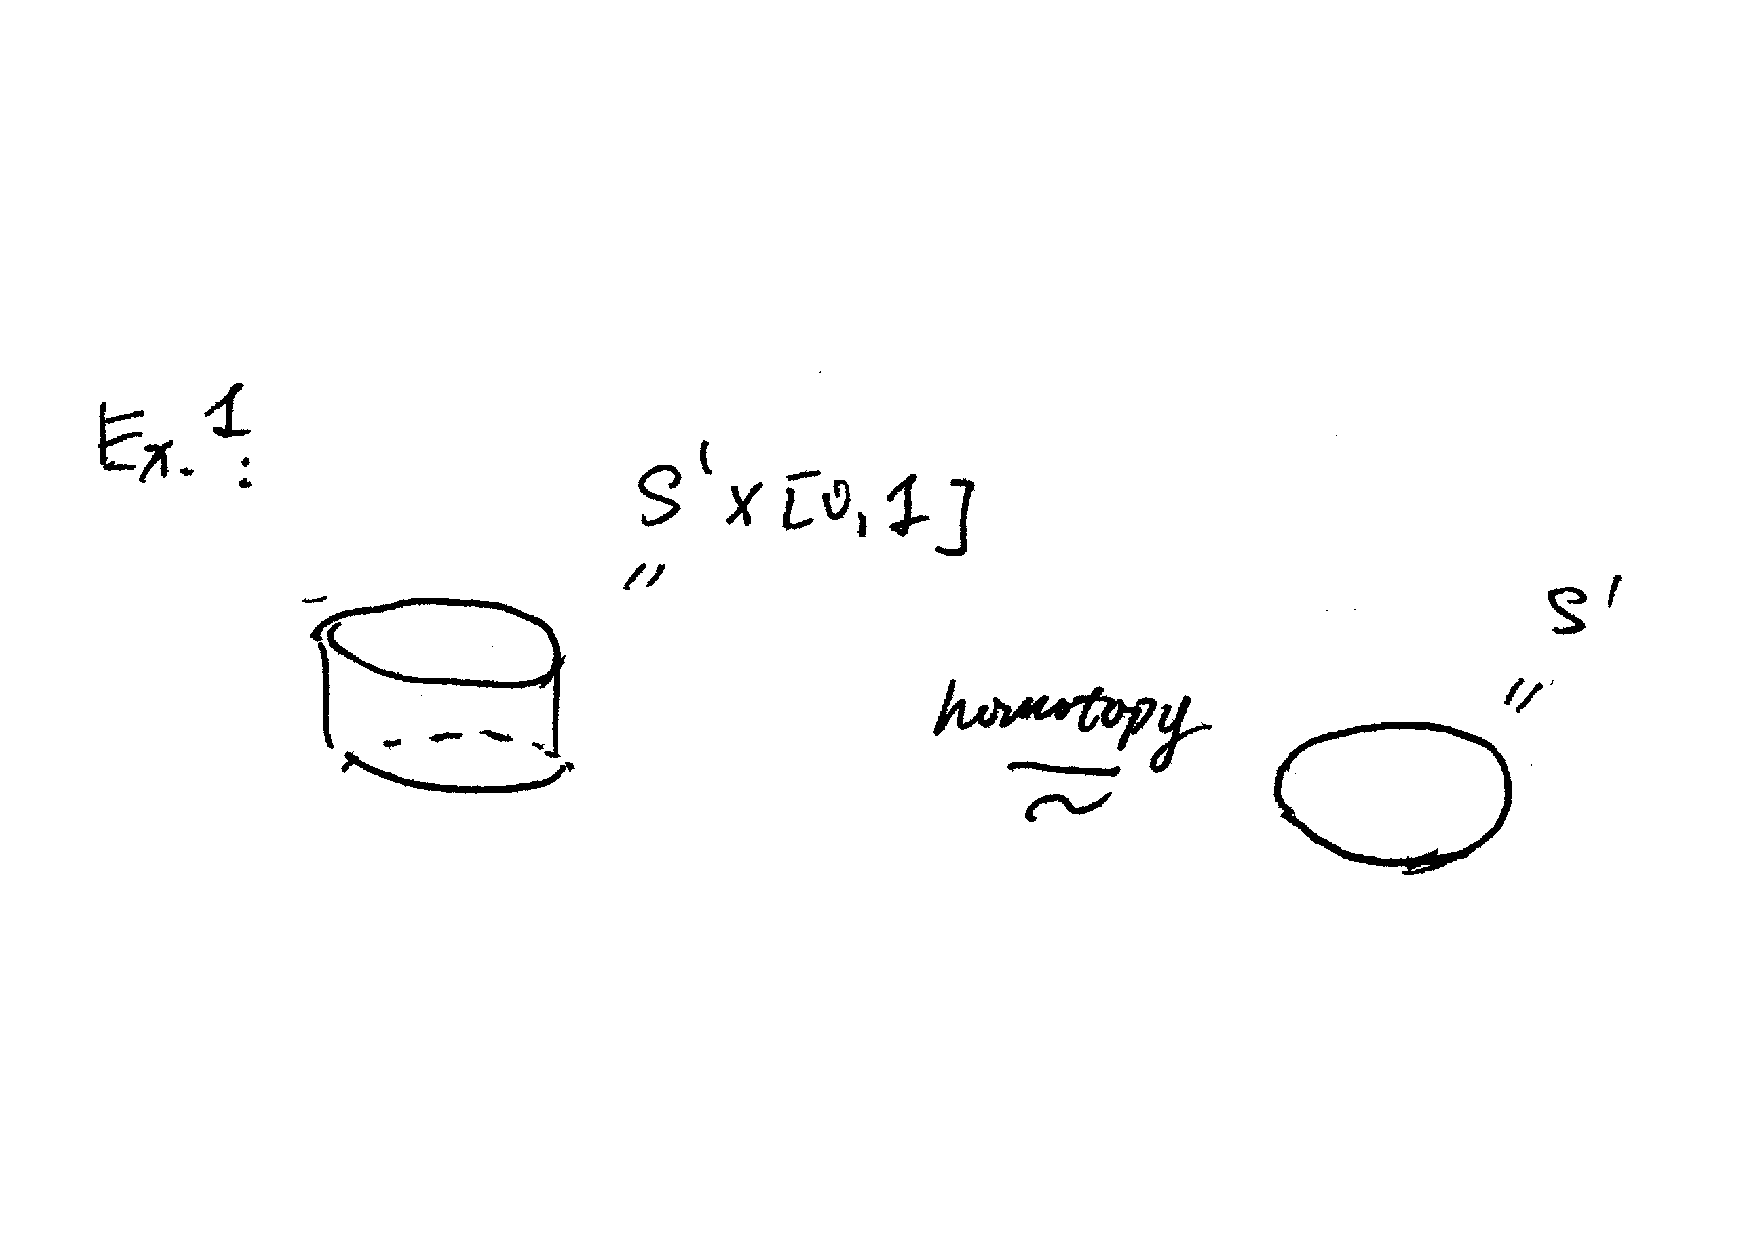
\includegraphics[width=0.6\linewidth]{pics/ch6-scanned-notes-1/ex1.pdf}
    \end{figure}
\end{ex}
\begin{ex}
    A non trivial one. That is, the M\"obius Strip also has the
    homotopy type of a ciclr $S^1$.
    \begin{figure}[H]
        \centering
        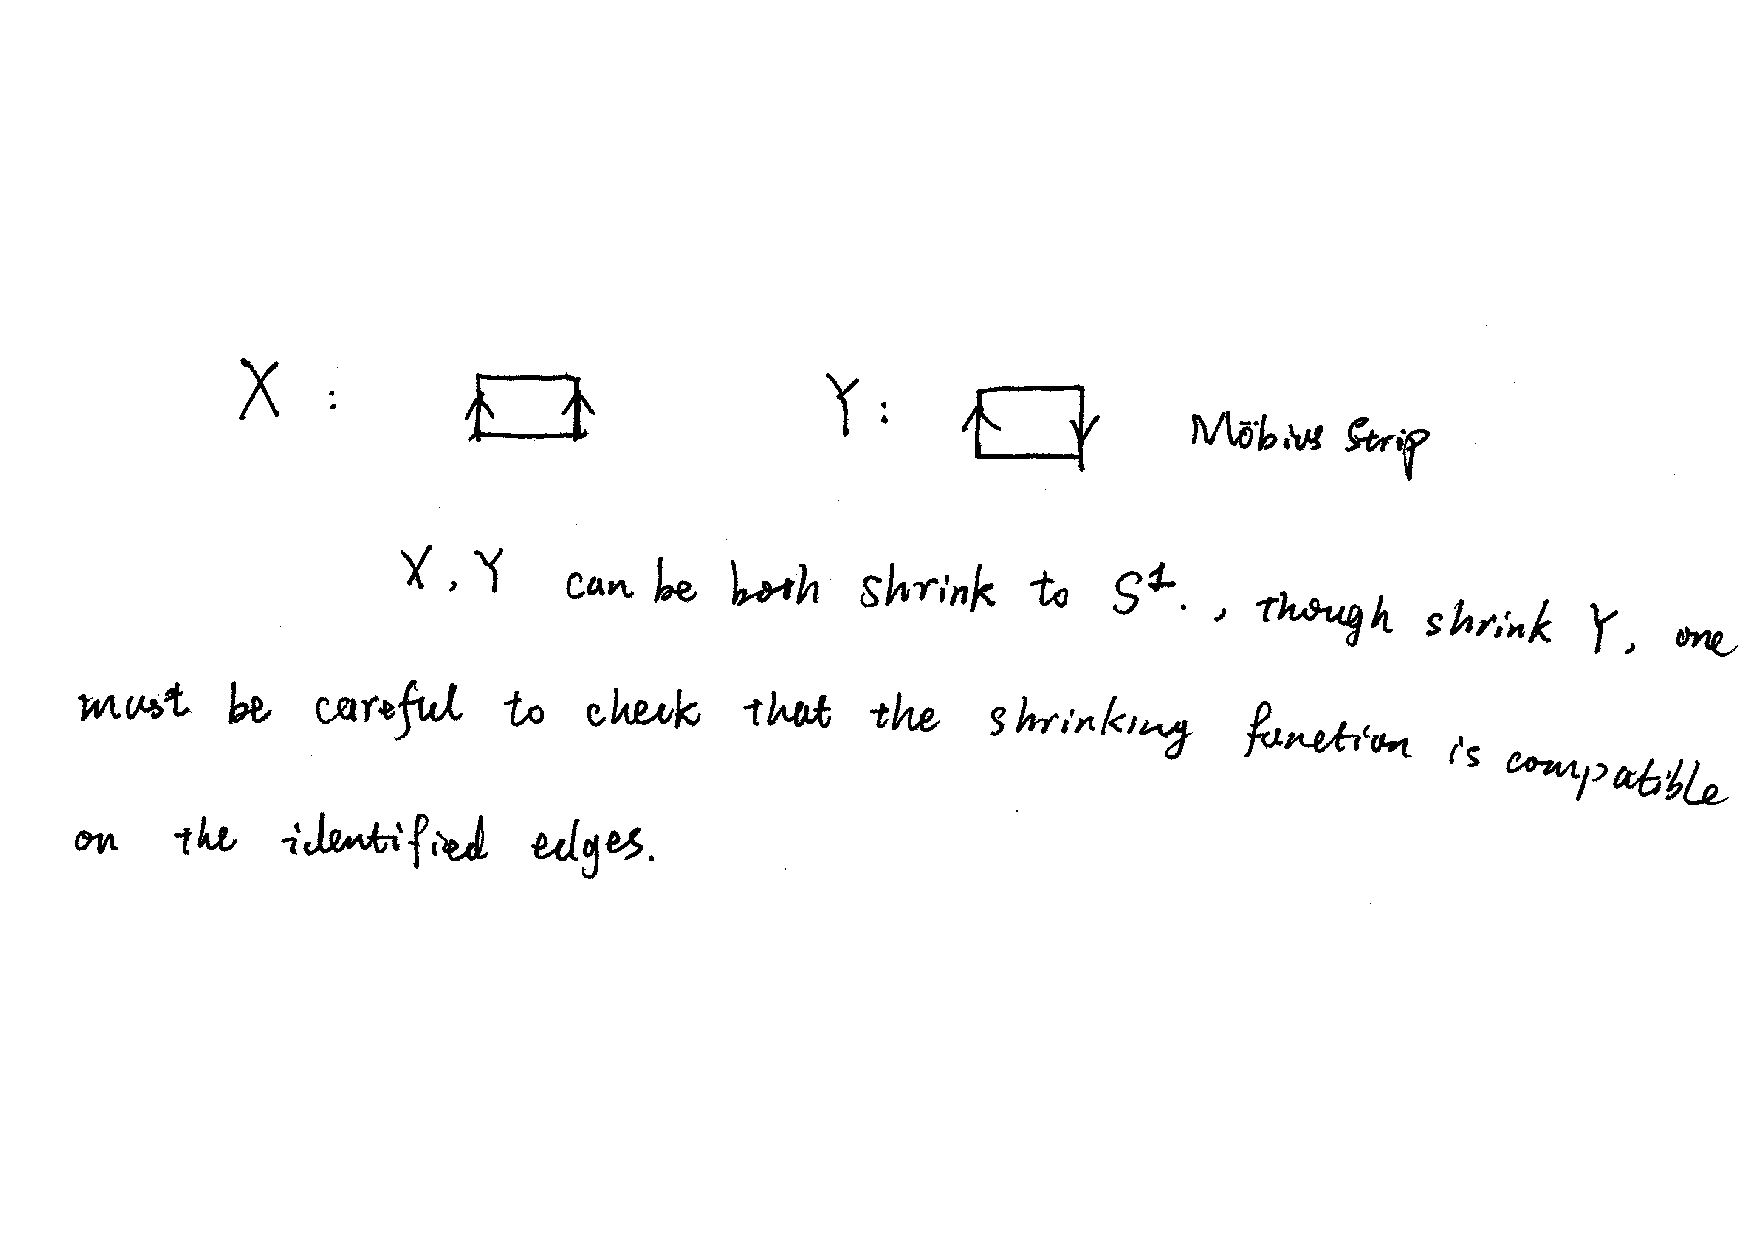
\includegraphics[width=0.8\linewidth]{pics/ch6-scanned-notes-1/ex2.pdf}
    \end{figure}
\end{ex}
But for complicated spaces, its homotopy type will not be so easy to
calculate in with simple imagination. Here we will introduce a new
technique to actually calculate the homotopy type of topological
spaces.

The technique is called Triangulation. The most visual example comes
from the computer vision technology (though I cannot find a picture by
directly Googling triangulation). The idea we wants to stress is that
the Triangulation is like use small patches of triangles to patch and
cover the surface of 3D smooth objects. Increase the overall number of
patches and make each patch get smaller. In the limit of this process
one might get to recover the original image.

\begin{defi}[Simplex of $\dim k$]
\nomenclature{Simplex of $\dim k$}{\nomrefpage.}
    The stanford simplex of $\dim k$ in $R^{k+1}$ is defined as
    follows. Let $v_i=(0,\cdots,0,1,0,\cdots 0)$, where $1$ is in $i+1$
    coordinates. That is:
    $$ v_0=(1,0,\cdots)$$
    $$ v_1=(0,1,0\cdots)$$
    $$\cdots$$
    $$ v_0=(0,\cdots,0,1)$$
    Then the simplex is the smallest convex set containing
    $\{v_0,\cdots,v_k\}$ in $\R^{k+1}$. It is also called a
    \nomen{$k$-simplex}.
\end{defi}
\begin{ex}
    \begin{figure}[H]
        \centering
        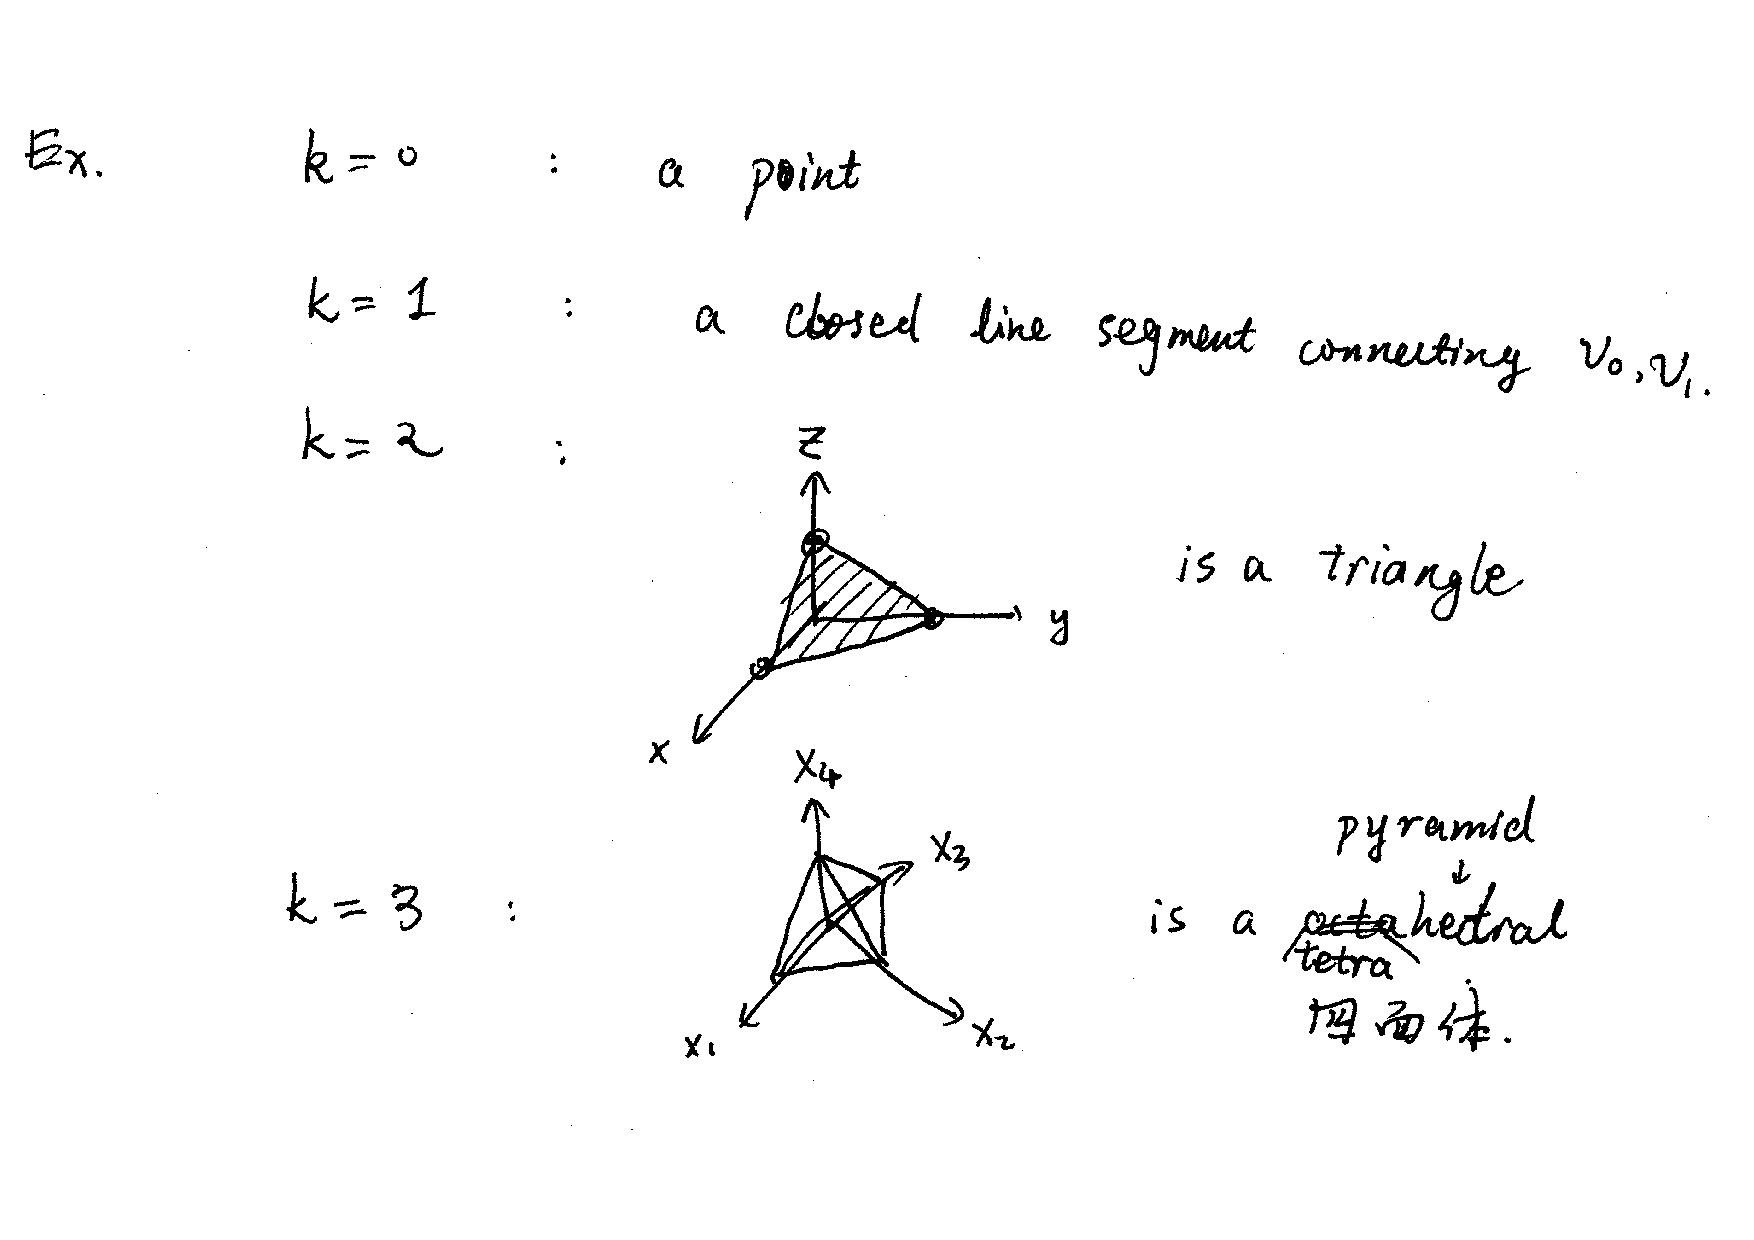
\includegraphics[width=0.8\linewidth]{pics/ch6-scanned-notes-1/ex3.pdf}
    \end{figure}
\end{ex}
\begin{fact}
    Any point in a $k$-simplex is of the form:
    \begin{equation}
        \lambda_0 v_0 + \lambda_1 v_1 + \cdots + \lambda_k v_k
    \end{equation}
    where each $\lambda_i\geq 0$, and $\sum_{i=0}^{k} \lambda_k=1$.
\end{fact}
\begin{ex}
    There is a special point in the $k$-simplex:
    \begin{equation}
        \frac{1}{k+1} \sum_{i=0}^k v_i
    \end{equation}
    When $k=2$, this is just the usual center of gravity of triangle.
\end{ex}

We want to study those space which is the union of a finite collection
of simplexes which fit together nicely in some Euclidean space. These
are called "triangulable spaces". More specifically:
\begin{defi}[faces]
\nomenclature{faces}{\nomrefpage.}
    If $A$ and $B$ are simplexes, and if the vertices of $B$ form a
    subset of vertices of $A$. Then $B$ is called a face of $A$,
    written as \nomen{$B<A$}.
\end{defi}
\begin{defi}[Simplicial Complex]
\nomenclature{Simplicial Complex}{\nomrefpage.}
    A \textbf{finite} collection of simplexes in some Euclidean space
    in $\R^n$ is called a simplicial complex, if
    \begin{enumerate}
        \item whenever a simplex lies in this collection, then so does
            its faces
        \item whenever two simplexes in this collection intersect,
            their intersection is a common face of these two
            simplexes.
    \end{enumerate}
\end{defi}
\begin{ex}
    % ex 4
\end{ex}
\begin{defi}[Topology on simplicial complex]
\nomenclature{Topology on simplicial complex}{\nomrefpage.}
    The topology on a simplicial complex is given by the subspace
    topology of Euclidean space. Let $K$ be a simplicial complex, we
    denote \nomen{$|K|$} as the topology of $K$. This $|K|$ is called
    a \nomen{polyhedron}.
\end{defi}

\begin{defi}[Triangulation and Triangulable]
\nomenclature{Triangulation and Triangulable}{\nomrefpage.}
    A triangulation on a topological space $X$ consists of a
    simplicial complex $K$, and a homeomorphism $h$:
    $$ h:|K|\to X$$
    A space is called triangulable if such simplicial complex $|K|$
    and homeomorphism $h$ exists.
\end{defi}
\begin{fact}
    If $X$ is triangulable, then $X$ is compact and can be made into a
    metric space. (Notice that the simplicial complex is a finite
    collection.)
\end{fact}
\begin{remark}
    Trigulation is in general not unique. For example:
    \begin{figure}[H]
        \centering
        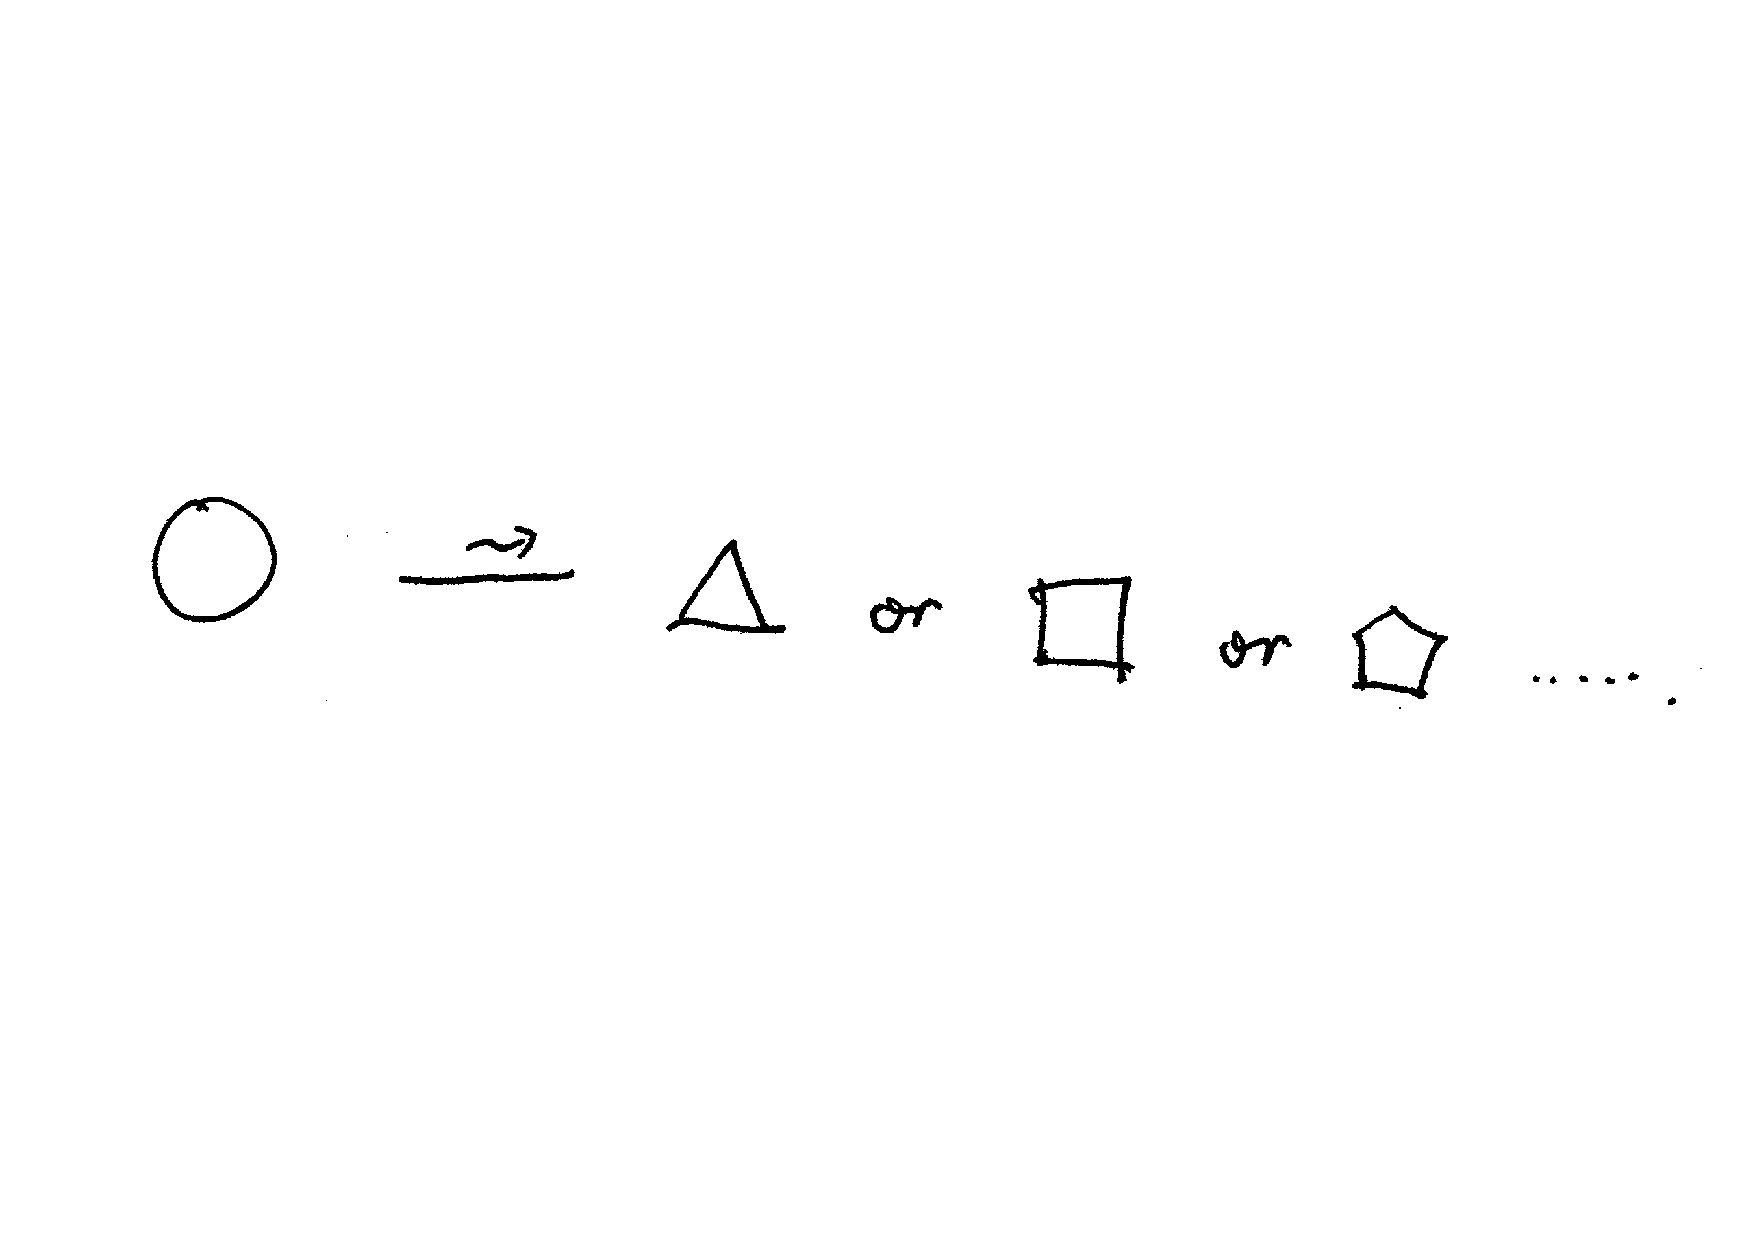
\includegraphics[width=0.6\linewidth]{pics/ch6-scanned-notes-1/rmk2}
    \end{figure}
\end{remark}
\begin{ex}
    Here is a triangulation on the torus:
    \begin{figure}[H]
        \centering
        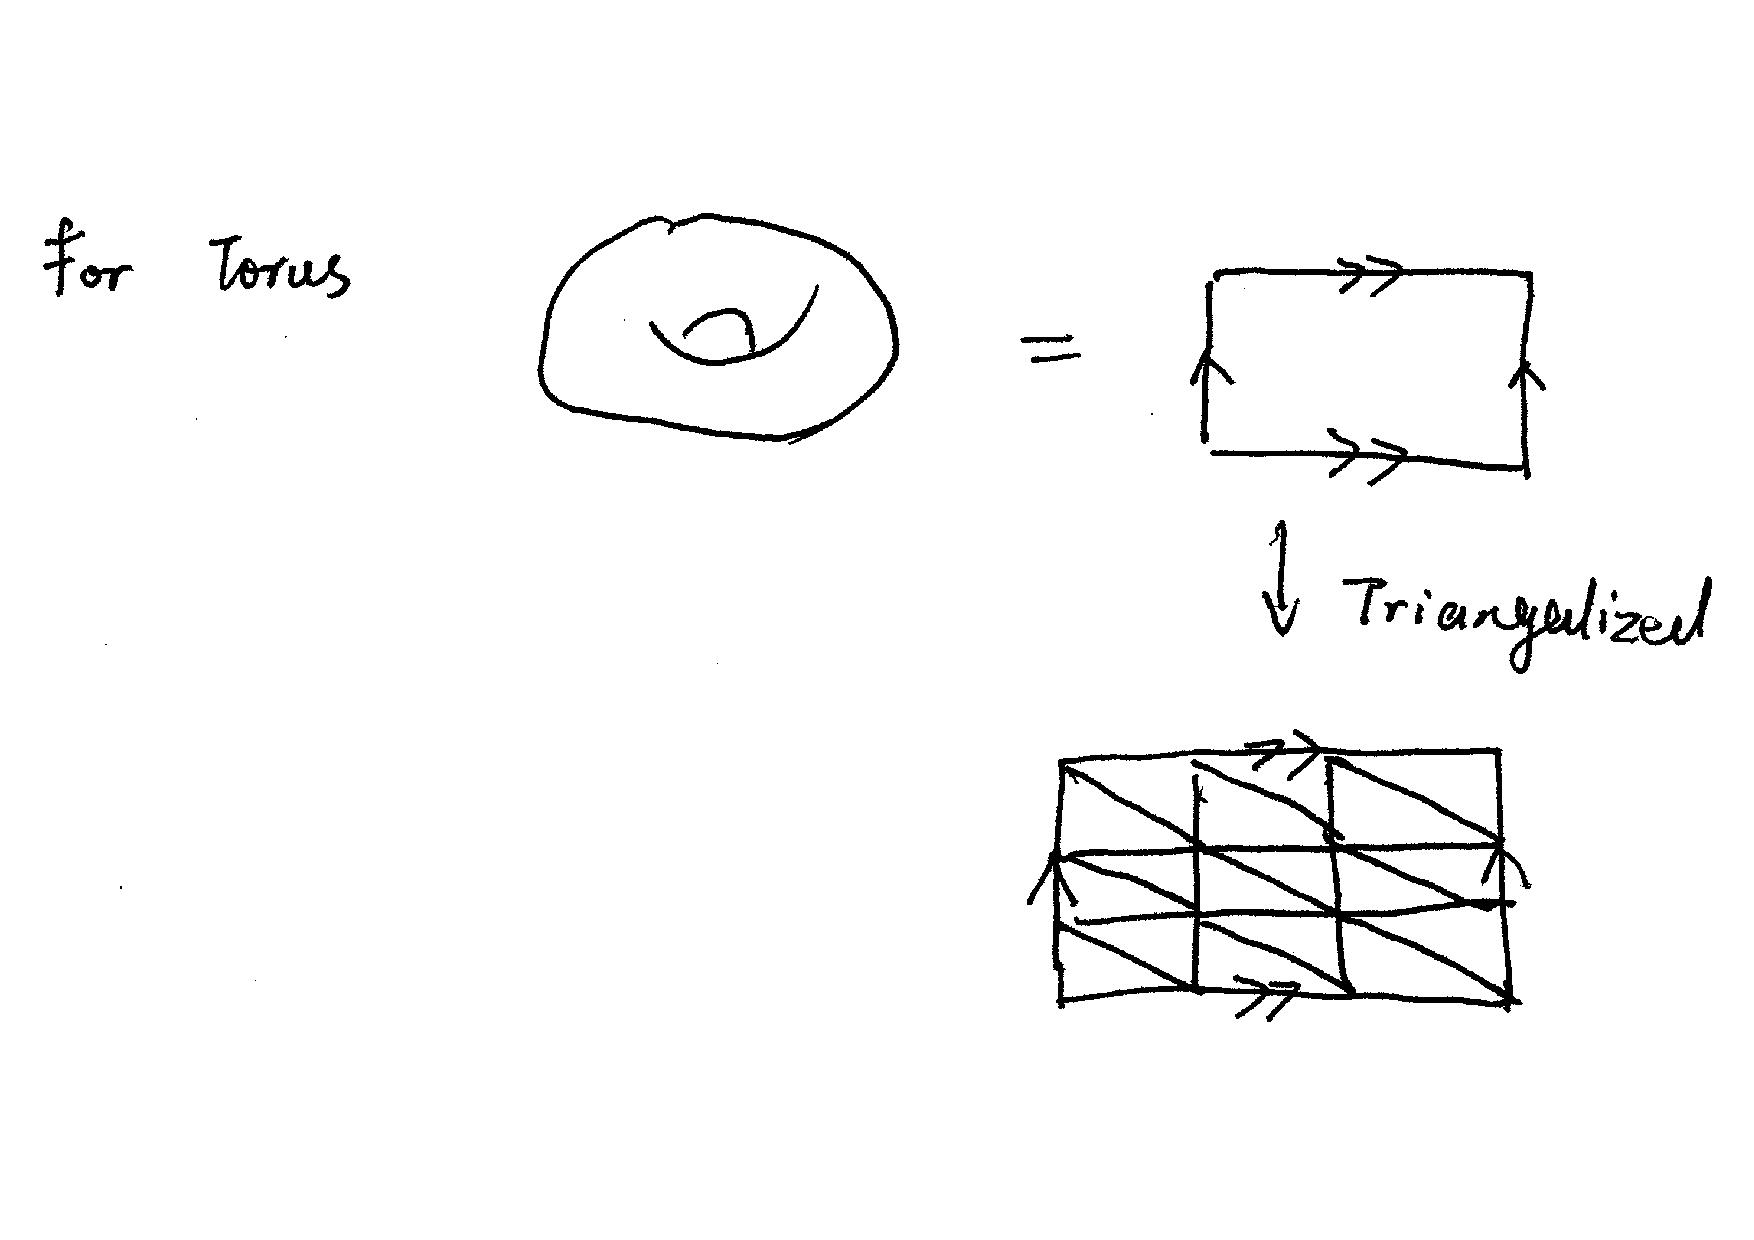
\includegraphics[width=0.6\linewidth]{pics/ch6-scanned-notes-1/p5.pdf}
    \end{figure}
    Notice that the following diagram is not a triangulation of torus:
    \begin{figure}[H]
        \centering
        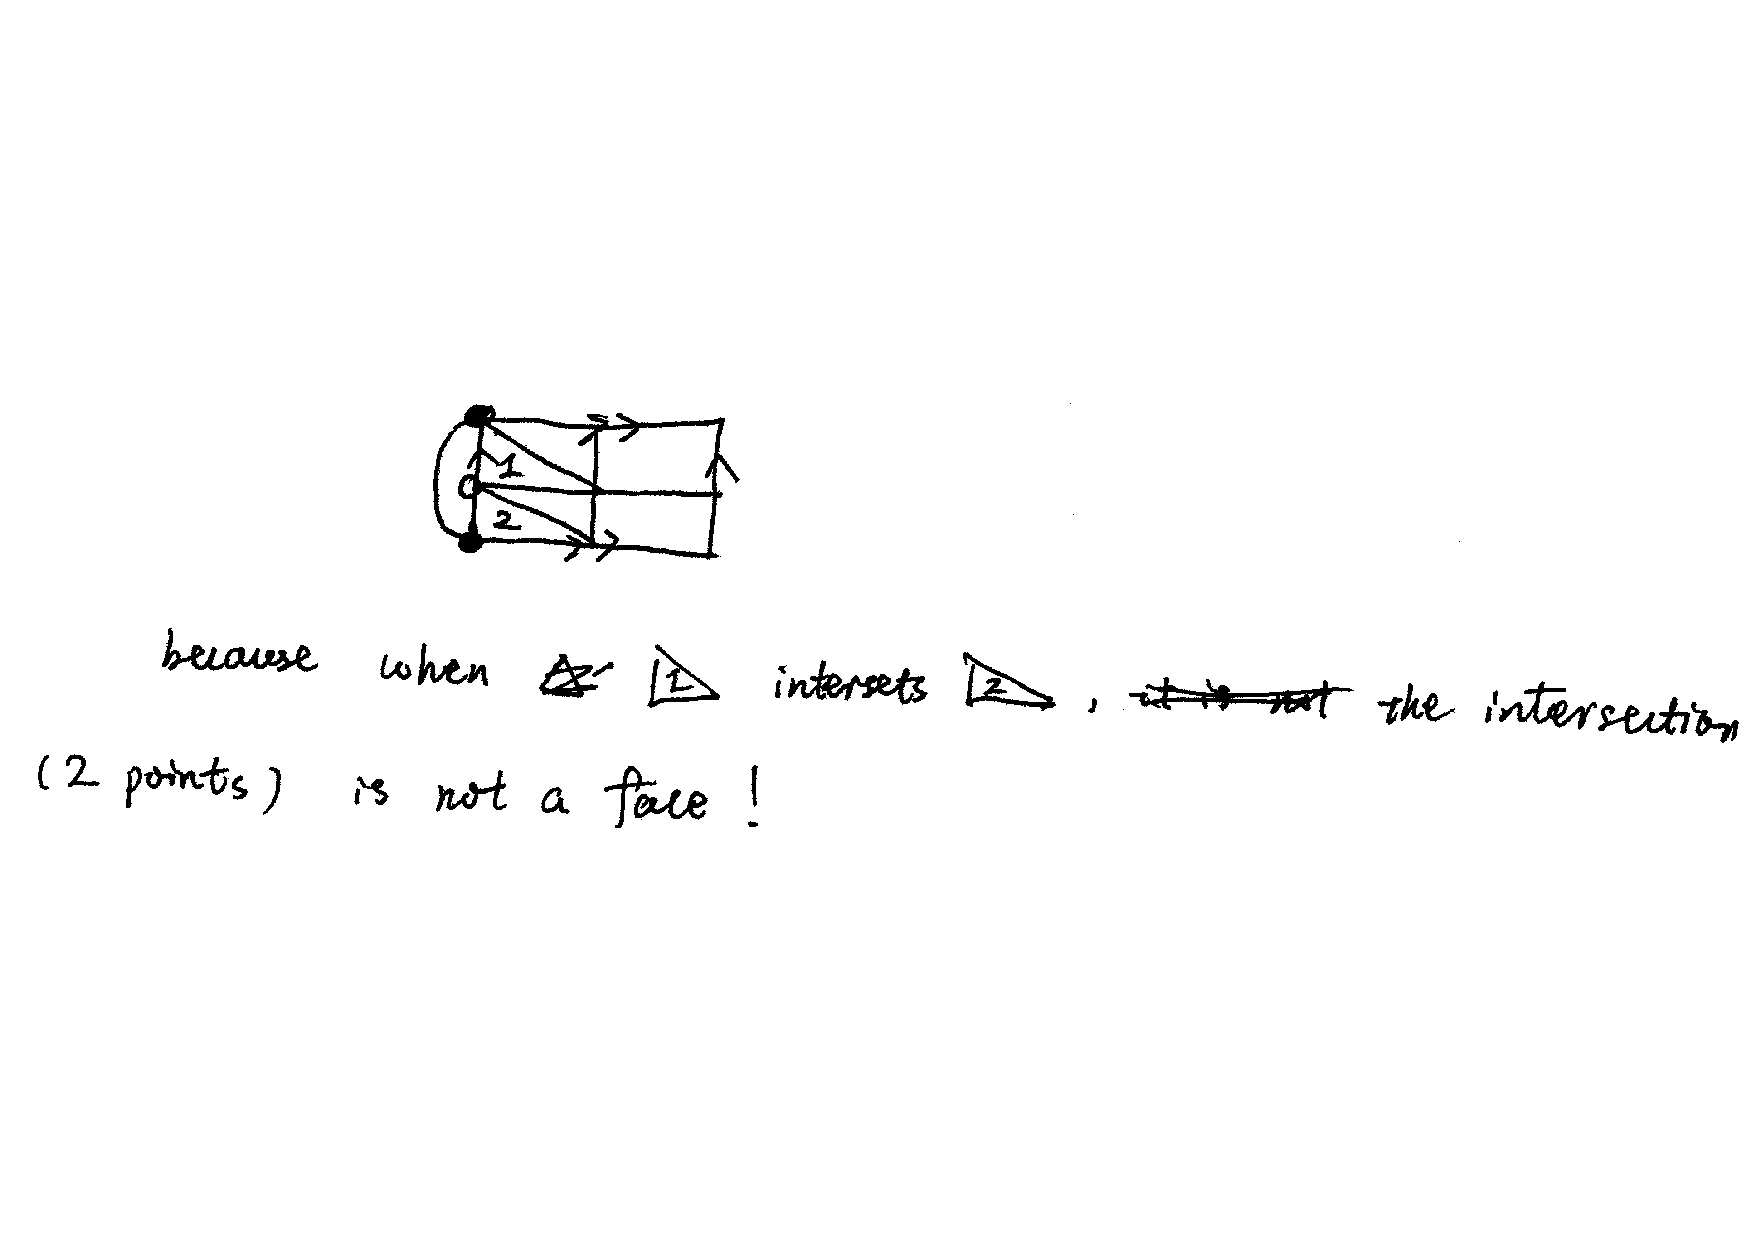
\includegraphics[width=0.8\linewidth]{pics/ch6-scanned-notes-1/p52.pdf}
    \end{figure}
\end{ex}
\begin{lemma}
    Let $K$ be a simplicial complex in $\R^{n}$, then
    \begin{enumerate}
        \item $|K|$ is compact.
        \item Each point of $|K|$ lies in the interior of exactly one
            simplex of $K$.
        \item If we take the simplexes of $K$ seperately, and give
            their union the identification topology, we obtain $|K|$.
            Thus we have two equivalent ways to view the topology on
            $K$.
        \item If $|K|$ is connected, then $|K|$ is also
            path-connected.
    \end{enumerate}
\end{lemma}
\begin{proof}
\begin{enumerate}
    \item Obviously.
    \item Since $K$ is connected by simplexes, a point $p$ must
        obviously be contained in some simplex. Also, since on each
        simplex $p$ must be on the interior of it, or interior of its
        components. We only need to prove that the containing simplex
        is unique. Suppose $p$ is the interior of simplexes $A$ and
        $B$. Notice that their intersection must be their faces. The
        only face of $A$ or $B$ containing interior points is $A$ or
        $B$ itself. Hence $A=B$.
    \item By definition of identification topology, we can see that in
        the identified space, a subset $C\subset |K|$, $C$ is closed
        $\Leftrightarrow$ $C\cap |A|$ is closed in $|A|$ for all
        simplexes $A\in K$. The rest of the proof is obvious.
    \item We need only to show that $|K|$ is locally path-connected.
        But any point $p\in K$, $p\in$ interior of some $A$ where
        $A\in K$. That is, we can find a neighbourhood $U$ of $p$, and
        $U$ is contained in $A$ ($U\subset A$). (More specifically, we
        can find $\varepsilon$ such that 
        $B_{\varepsilon}(p)\cup |K| = B_\varepsilon(p)\cup |A|$)
        But a simplex $A$ is obviously locally path-connected. Hence
        $U$ (or $B_\varepsilon(p)$) is path connected, hence $|K|$ is
        path-connected.
\end{enumerate}
\end{proof}

\subsection{Section 6.2 Barycentric Division}
\label{sec:Barycentric-Division}
Now we begin to make the triangulation more and more detailed. We
start from a simplicial complex $K$ and constructing a new simplicial
complex $K_1$, such that
\begin{enumerate}
    \item $|K|=|K_1|$, homeomorphically.
    \item diameter $|K_1|<$ diameter $|K|$.
\end{enumerate}
The general construction method is called Barycentric division,
visualized as:
\begin{figure}[H]
    \centering
    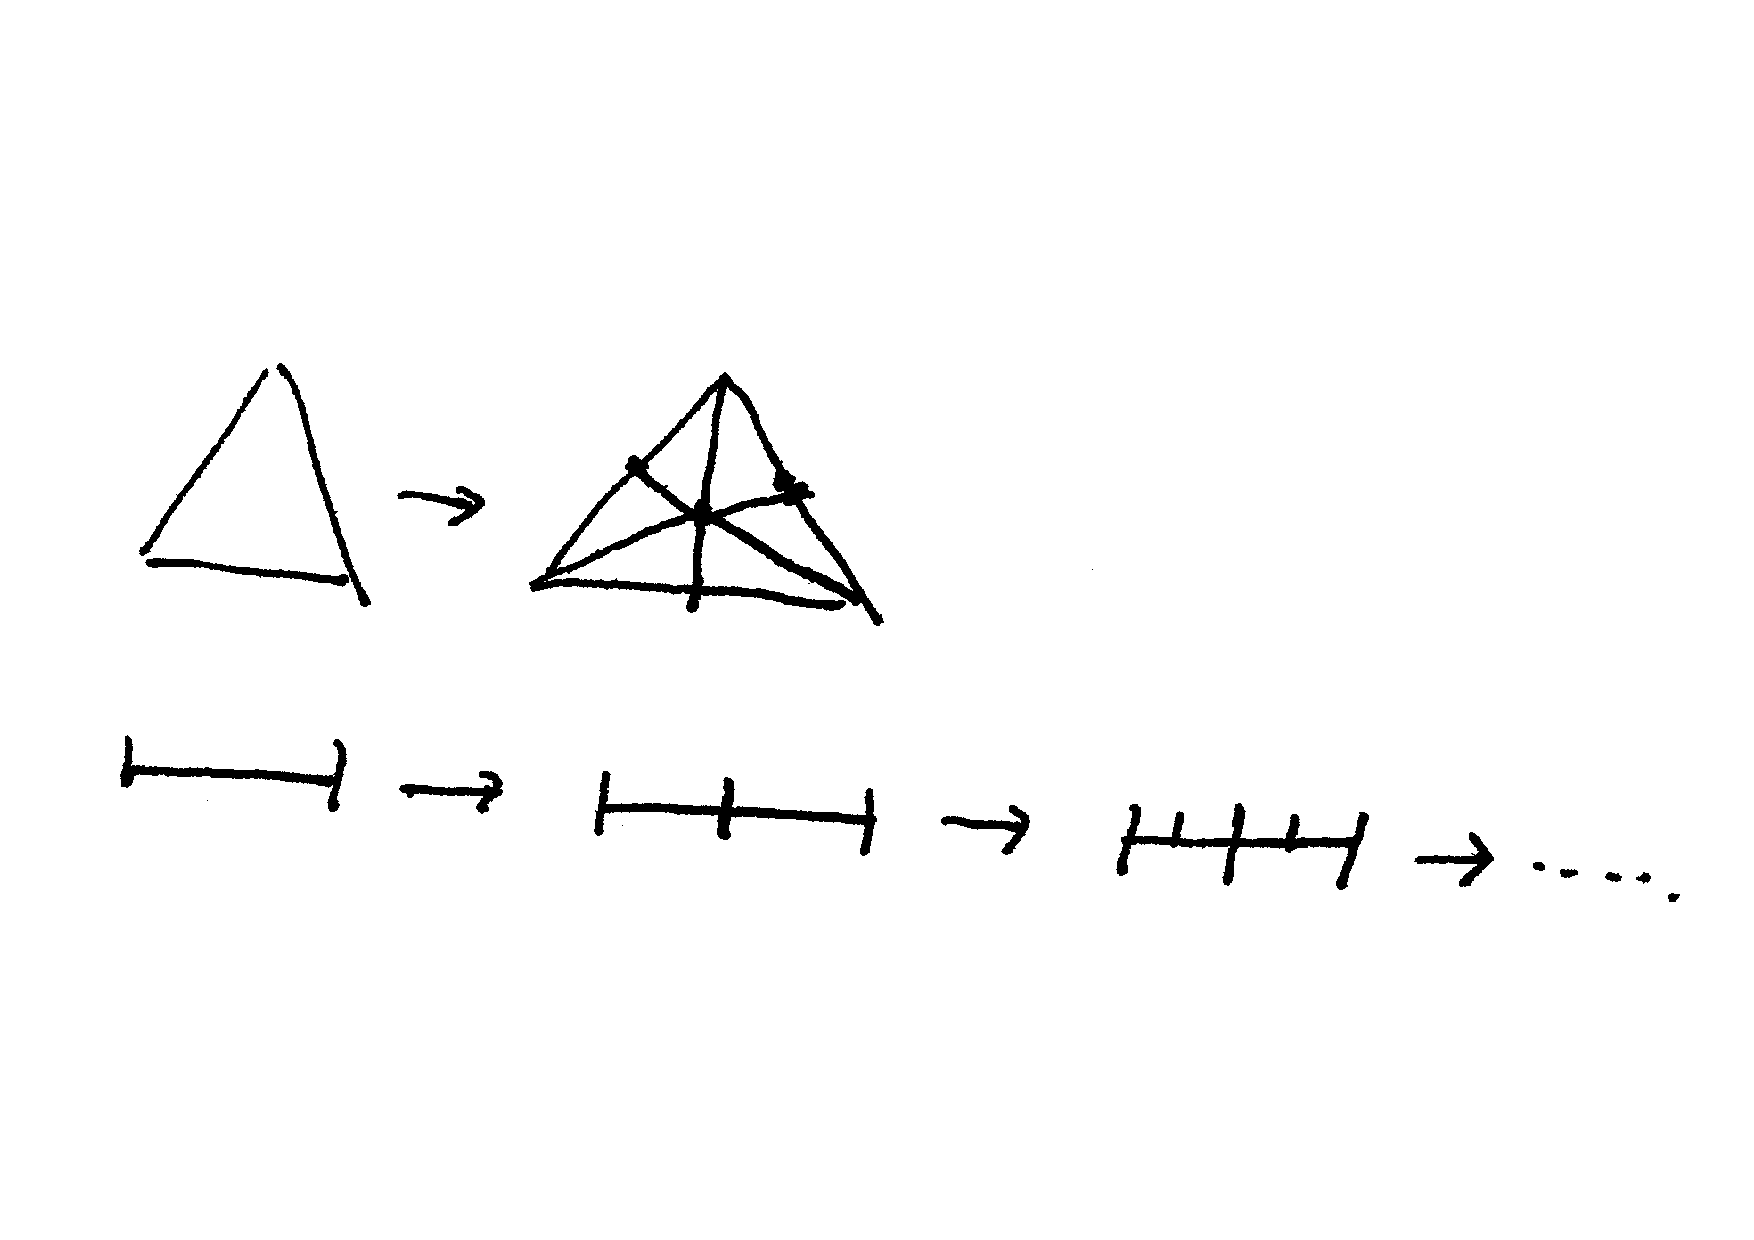
\includegraphics[width=0.6\linewidth]{pics/ch6-scanned-notes-1/8.pdf}
\end{figure}
We first define a concept
\begin{defi}[$\hat{A}$ Bary center]
\nomenclature{$\hat{A}$ Bary center}{\nomrefpage.}
Let $A$ be a simplex, then the bery center of $A$, denoted $\hat{A}$,
is the point:
\begin{equation}
    \hat{A}:= \frac{1}{k+1}(v_0+\cdots+v_k)
\end{equation}
\end{defi}
Then, the general process is:
The new space $K_1$ is such that
\begin{enumerate}
    \item The vertices of $K_1$ are bary centers of \textbf{ALL}
        simplexes of $K$. Note the the bary center of a $0$-simplex
        is just itself. So in general, $K_1$ has more vertices of
        $K$.
    \item A collection $\hat{A}_0,\cdots,\hat{A}_k$ of such bary
        centers will form a vertex of a $k$-simplex in $K_1$ if and
        only if there is a permutation $\sigma$ of $\{0,1,\cdots,k\}$
        such that
        \begin{equation}
            A_{\sigma{0}}< A_{\sigma{1}} < \cdots < A_{\sigma{k}}
        \end{equation}
\end{enumerate}
\begin{remark}
    The second point above tries to do the following
    \begin{figure}[H]
        \centering
        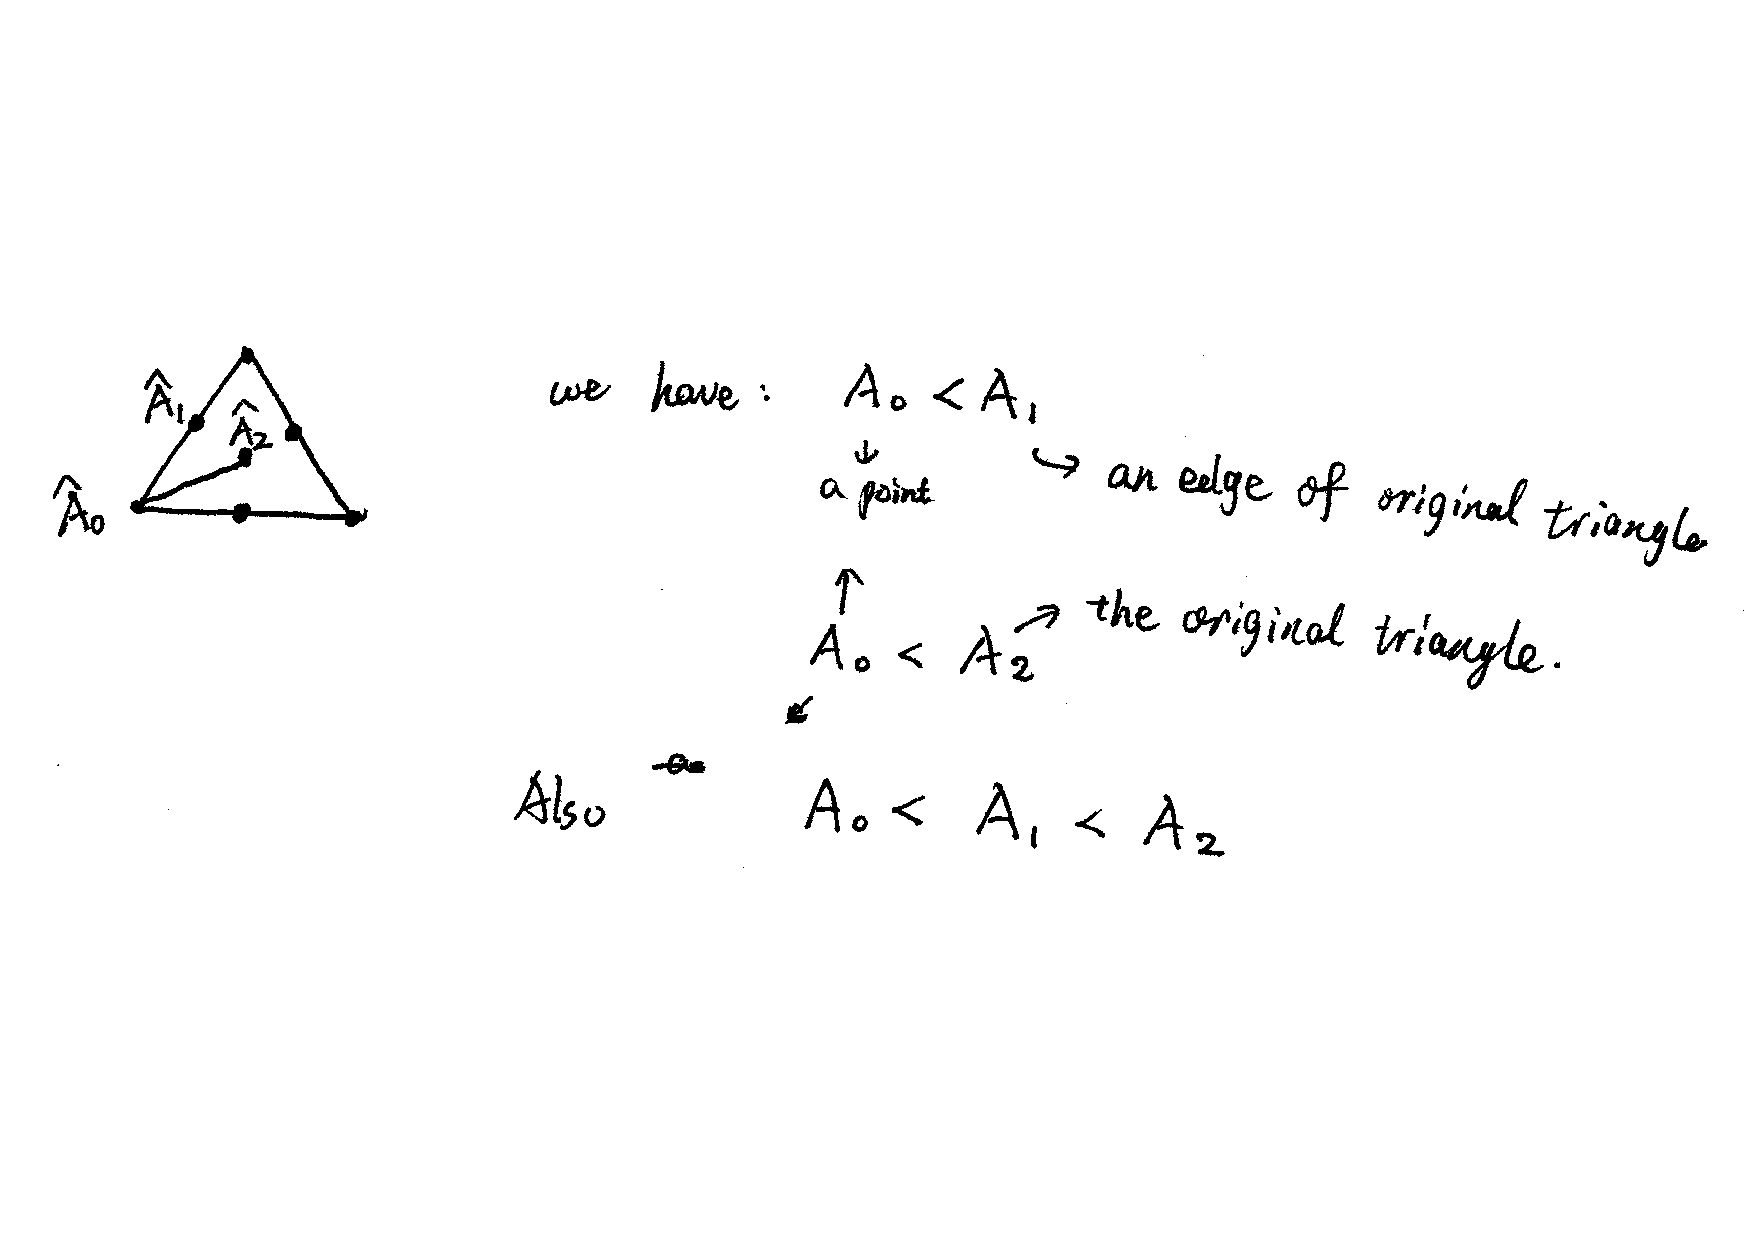
\includegraphics[width=0.9\linewidth]{pics/ch6-scanned-notes-1/p9.pdf}
    \end{figure}
\end{remark}

Now we give a precise description of how this Bary center division
will work. We first describe precisely two characteristics of a
simplicial complex. 

\begin{defi}[dimension of a simplicial complex]
\nomenclature{dimension of a simplicial complex}{\nomrefpage.}
    The dimension of a simplicial complex $K$ is the maximum of the
    dimensions of all its simplexes.
\end{defi}
\begin{defi}[mesh $\mu(K)$]
\nomenclature{mesh $\mu(K)$}{\nomrefpage.}
    The mesh of a simplicial complex $K$ is the maximum of the
    diameters of all its simplexes.
\end{defi}

As we expected, the mesh (which carries the intuition of the smallness
of one simplicial complex) of a simplicial complex will decrease. The
following lemma confirmed this.

\begin{lemma}
    The sollection of simplexes described above forms a simplicial
    complex. If it is denoted by $K^1$, and is called the first
    barycentric subdivision of $K$, then $K^1$ has the following
    properties:
    \begin{enumerate}
        \item each simplex of $K^1$ is contained in a simplex of $K$;
        \item Their topology are the same: $|K^1|=|K|$
        \item If the dimension of $K$ is $n$, then
            \begin{equation}
                \mu(K^1)\leq \frac{n}{n+1}\mu(K)
            \end{equation}
    \end{enumerate}
\end{lemma}
\begin{proof}
    The proof can be found in page 126 to 127 of \cite{book}. But the
    proof of the last point is not so clear and is illustrated here:
\begin{figure}[H]
    \centering
    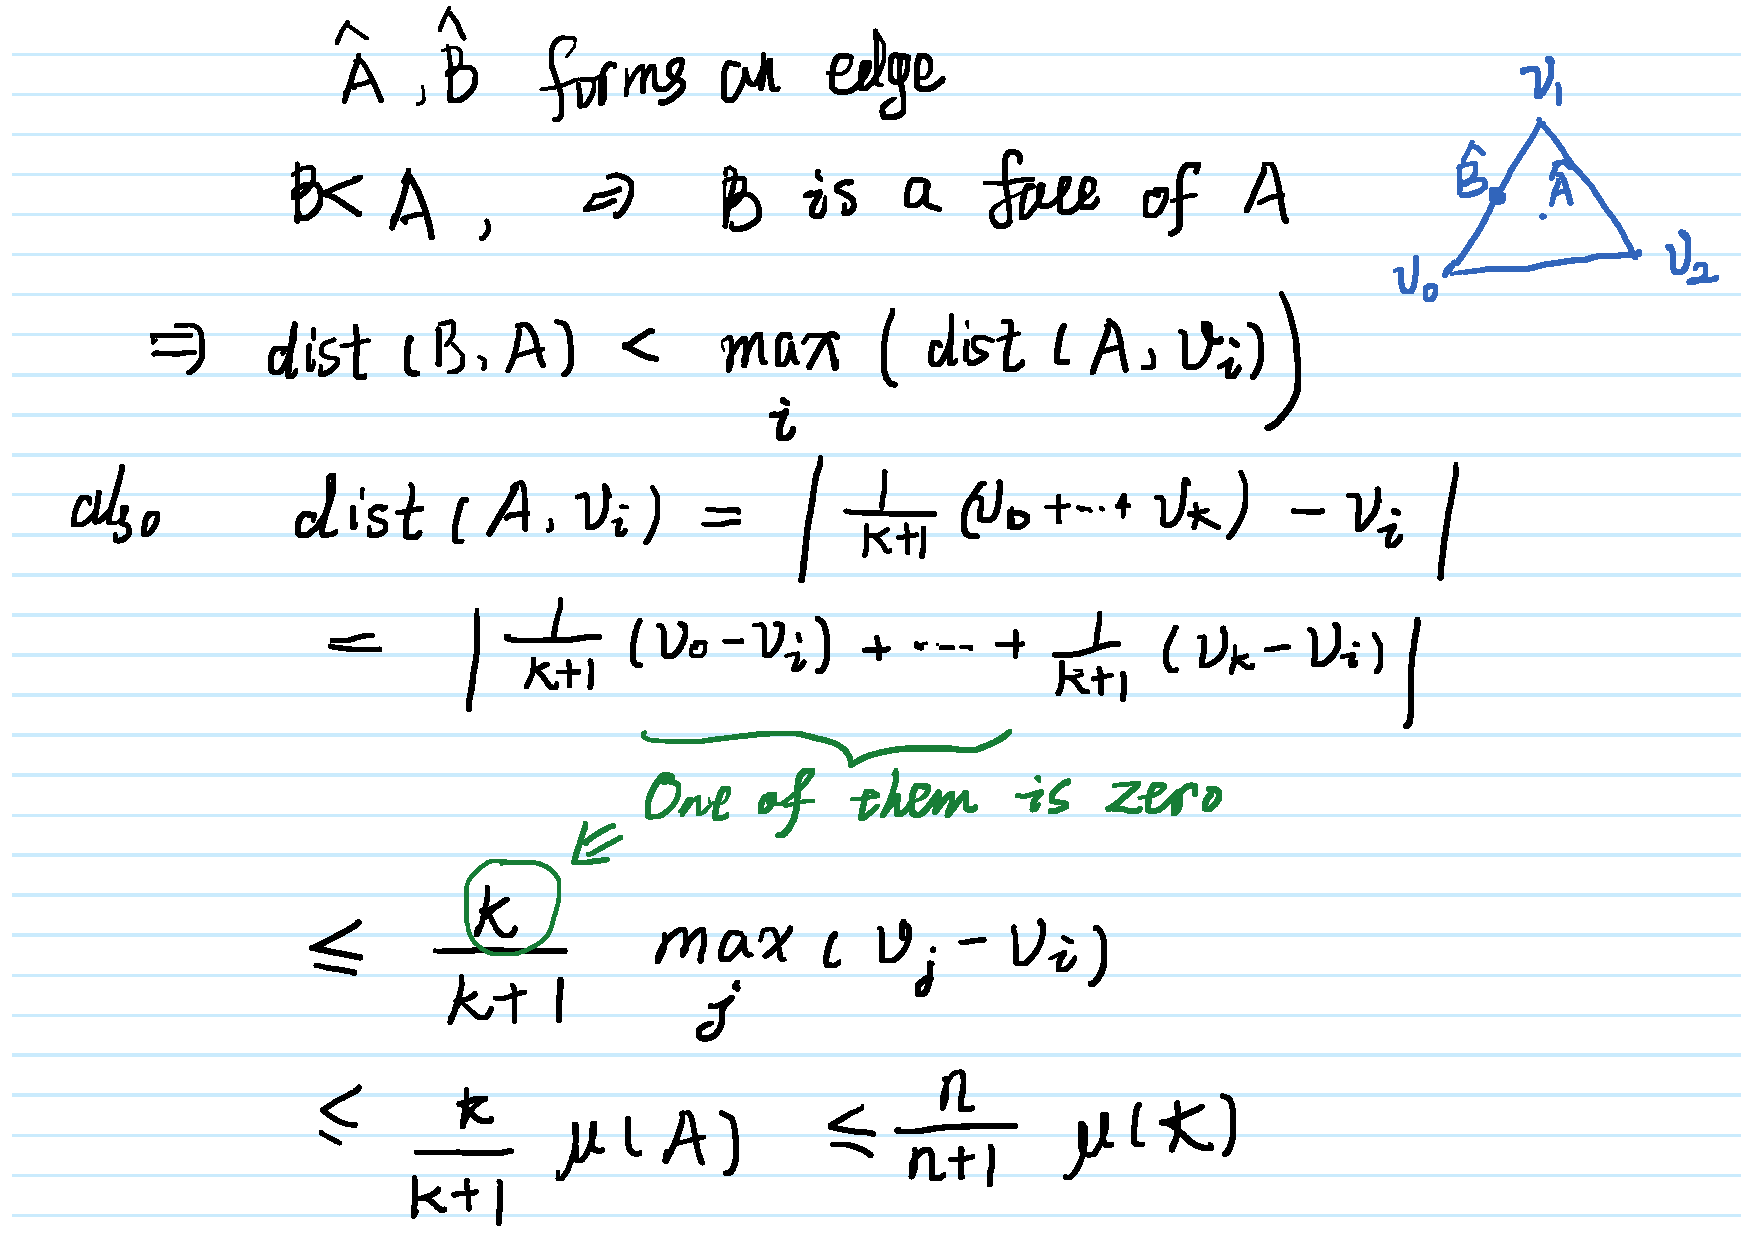
\includegraphics[width=1\linewidth]{pics/ch6-notes-2/explain1.pdf}
\end{figure}
\end{proof}
\begin{remark}
    Notice that the number $\frac{n}{n+1}<1$, hence after an infinite
    number of Barycentric subdivision, the mesh (averaged diameter) of
    a simplicial complex $K^m$ will goes to zero!
\end{remark}
\subsection{Section 6.3 Simplicial approximation}
\label{sec:Simplicial-approximation}

The purpose here is to approximate any continuous map $f:A\to B$ with
linear map, in a way that is compatible with the triangulations on
both $A$ and $B$.
\begin{figure}[H]
    \centering
    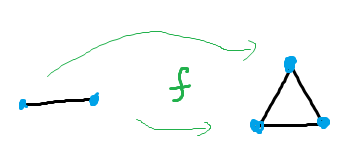
\includegraphics[width=0.4\linewidth]{pics/ch6-notes-2/exp2.png}
\end{figure}
\begin{defi}[Simplicial map]
\nomenclature{Simplicial map}{\nomrefpage.}
    Let $K$ and $L$ be simplicial complexes. A continuous map $s:K\to
    L$ is called simplicial, if it takes simplexes of $K$
    \textit{linearly} to simplexes of $L$. Specifically, being
    \textit{linear} means that:
    
    For $\forall A\in K$, we have $B=s(A)\in L$. Also, if
    $A=\{v_0,\cdots,v_k\}$, then $B=\{s(v_0),\cdots,s(v_k)\}$.
    Lastly, if $x=\sum_{i=0}^k \lambda_i v_i$ is a a point in $A$, with
    $\lambda_i\geq 0$ and $\sum_{i=0}^k\lambda_i=1$, then
    $$s(x) = \sum_{i=0}^k \lambda_i s(v_i)$$

    In a word, $s$ maps simplexes to simplexes, vertices, to vertices,
    and points linearly to points.
\end{defi}
\begin{remark}
    It is easy to see that the a simplicial map is uniquely determined
    by its value on all the vertices. By this, there can only be a
    finite number of such kind of maps, since there are only a finite
    number of vertices.
\end{remark}

Now we want to find such linear maps to approximate a give function
$f:|K|\to |L|$. Given a point $x\in |K|$, we define the
\nomen{carrier of $f(x)$} to be the unique simplex of $L$ that contain
$f(x)$ as its interior point.

\begin{defi}[Simplicial Approximation]
\nomenclature{Simplicial Approximation}{\nomrefpage.}
    A simplicial map $s:|K|\to |L|$ is called a simplicial approximation of
    $f:|K|\to |L|$ if and only if $s(x)\in$ carrier of $f(x)$,
    $\forall x\in |K|$.
\end{defi}
\begin{ex}
    Trivial examples:
\begin{figure}[H]
    \centering
    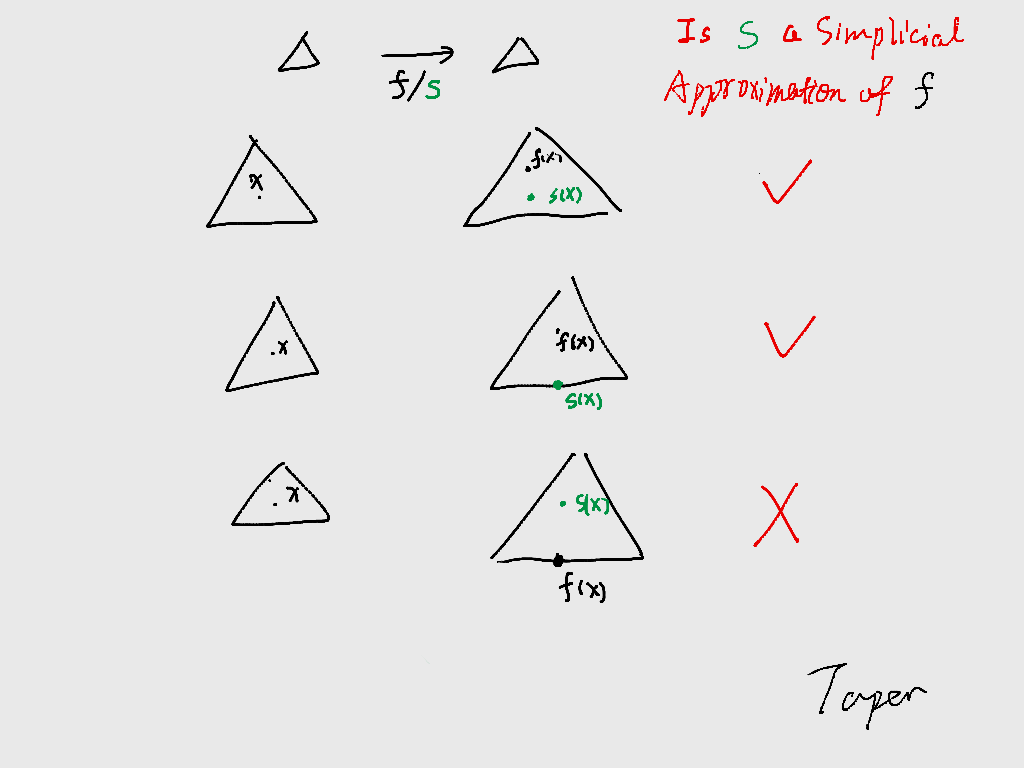
\includegraphics[width=0.8\linewidth]{pics/ch6-notes-2/ex3.png}
\end{figure}
\end{ex}
\begin{ex}
    Now we show that when simplicial approximation does not exits. The
    set up is as follows:
    \begin{figure}[H]
        \centering
        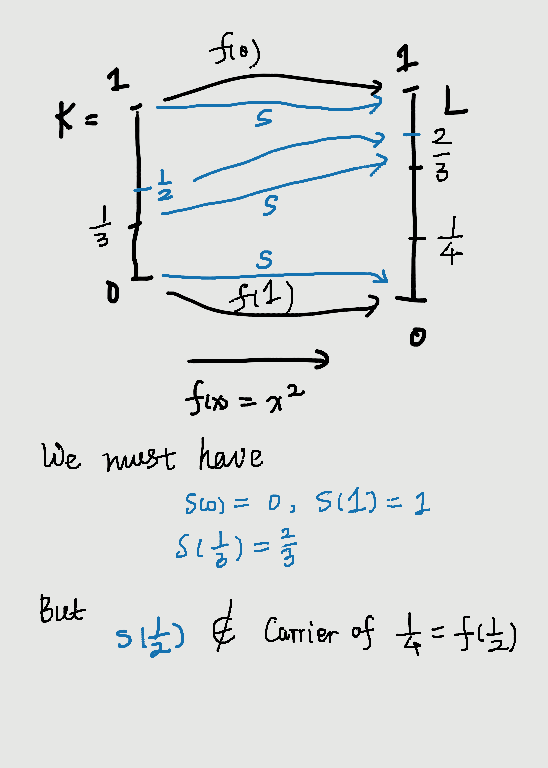
\includegraphics[width=0.8\linewidth]{pics/ch6-notes-2/ex4.png}
    \end{figure}
    Hence, there is no simplicial approximation of $f$. But, it will
    be shown below that, if we divide $K$ small enough
    ($K^1,K^2,\cdots$), we will eventually be able to find a
    simplicial approximation of $f$ in some $K^n$.
\end{ex}

\begin{thm}[Simplicial approximation theorem]
    \label{thm:SAT}
    Let $f:|K|\to |L|$ be a continuous map between polyhedras formed
    by simplicial complexes $|K|$ and $|L|$. If $m$ is chosen large
    enough, then there is a simplicial approximation $s:|K^m|\to|L|$
    to $f:|K^m|\to|L|$.
\end{thm}
The proof will use a lemma. Define the \nomen{open star} $v$ of a
simplicial complex $K$, as the union of the interiors of those
simplexes of $K$ having $v$ as a vertex. This union is denoted by
\nomen{$\operatorname{star}(v,K)$}. An example is:
\begin{figure}[H]
    \centering
    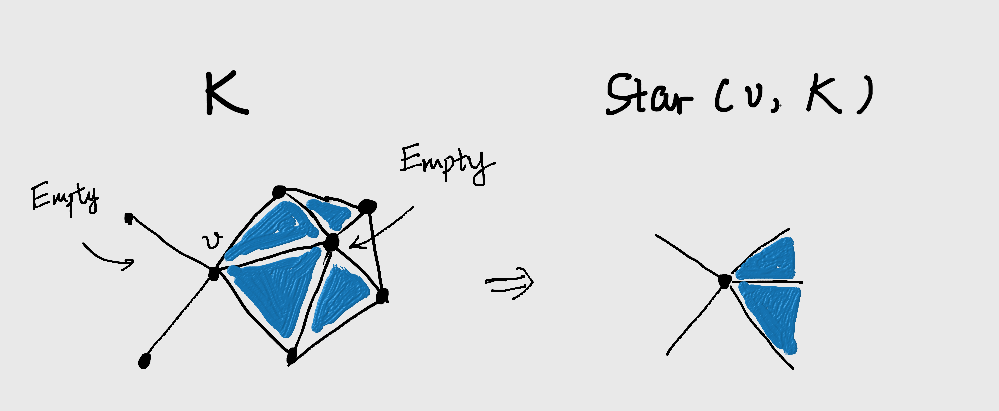
\includegraphics[width=1.0\linewidth]{pics/ch6-notes-2/ex5.png}
    \caption{Example of star}
\end{figure}
So it really feels like a star spreading out from $v$. We have

\begin{lemma}
    Vertices $v_0,v_1,\cdots,v_k$ of a simplicial complex $K$ are the
    vertices of a simplex of $K$ if and only if the intersection of
    their open stars is nonempty, i.e. 
    $$\cup_0^k \operatorname{star}(v_i,K)\neq\emptyset$$
\end{lemma}
\begin{proof}
    The proof can be found in page 130 of \cite{book}. It is quite
    trivial.
\end{proof}
Then we have the \textbf{proof of theorem \ref{thm:SAT}}:
\begin{proof}
    The proof is found in page 130 to 131 of \cite{book}. The idea is
    that if for each vertex $u$ of $K$, we can find a vertex $v$ of
    $L$ such that
    \begin{equation}
        f(\operatorname{star}(u,K))\subseteq\operatorname{star}(v,L)
        \label{eq:proof-temp} \tag{*} 
    \end{equation}
    Then the simplicial map $s(u)=v$ will be easily verified to be a
    simplicial approximation of $f$. 
    
    To make such (*) happen, we naturally have to divide $K^m$ small
    enough. We can achieve such small division is guaranteed by the
    Lebesgue lemma \ref{lemma:lebesgue-lemma}, since each subdivision
    makes the averaged diameter smaller.
\end{proof}

\subsection{Section 6.4 The edge group of a complex}
\label{sec:edge-group}

The definition of edge group is so similar to that of fundamental
group (actually, edge group is made to simplify computation of
fundamental group). Therefore, I will not waste too much words here.
One with reasonable intuition could just skim through this section.

The following excerpt from book \cite{book} best captures the idea:

\begin{myquote} \enquote{
We calculated the fundamental groups of one or two spaces in Chapter
5, but our calculations, though efficient for the examples given
there, were rather \textit{ad hoc}. If we agree to work with triangulable
spaces, we can be much more systematic. We shall show how to read off
generators and relationst for the fundamental group from a
triangulation of the space.

Let $X$ be a path-connected triangulable space, take a specific
triangulation $h:|K|\to X$, and replace $X$ by $|K|$ (we are at
liberty to do this since the funda- mental group is a topological
invariant). Now the advantage of a polyhedron $|K|$ is that the
elements of its fundamental group can be represented by loops which
are made up of edges of $K$. Using such 'edge loops' we shall
construct a group, called the edge group of the complex $|K|$, which
can be computed and wh ich is isomorphic to the fundamental group of
$|K|$.
} \end{myquote}

The edge pathes $v_0,v_1,\cdots,v_k$, edge loops
$v,v_1,\cdots,v_{k-1},v$ are defined similar to pathes and loops.
The equivalence relation between edge loops are defined as represented
by the following drawing:
\begin{figure}[H]
    \centering
    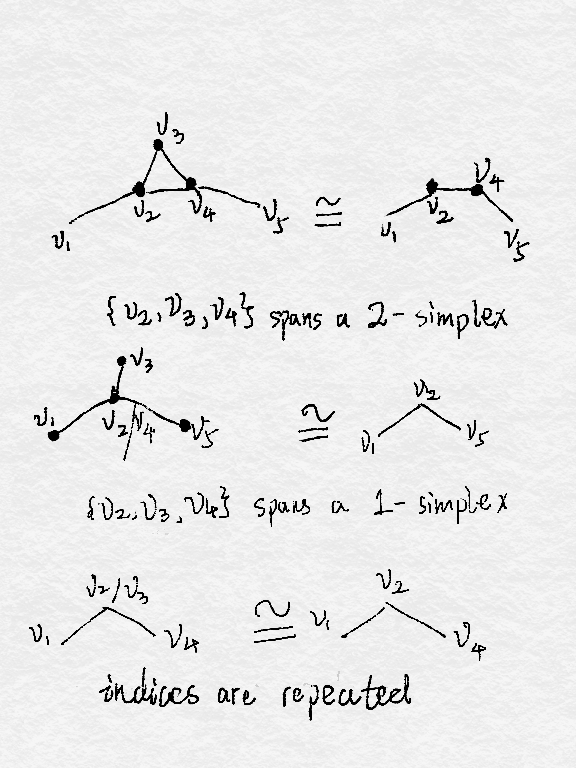
\includegraphics[width=0.8\linewidth]{pics/ch6-notes-2/edge-group1.png}
\end{figure}

The equivalence class of edge pathes and edge loops are denoted
$\{v_0,v_1,\cdots,v_k\}$, and $\{v,v_1,\cdots,v_{k-1},v\}$,
respectively. The multiplication of edge loops is defined simply as
\begin{equation}
    \{v,v_1,\cdots,v\}\{v,w_1,\cdots,v\} =
    \{v,v_1,\cdots,v,w_1,\cdots,v\}
\end{equation}

It is trivially verified that such edge loops form a group, called the
\nomen{edge group based at $v$, $E(K,v)$}. It is also trivially
verified that such group does not depend on the choice of base point
$v$, since $|K|$ is path-connected.

\begin{thm}
    $E(K,v)$ is isomorphic to $\pi_1(|K|,v)$
\end{thm}
\begin{proof}
    The proof can be found on page 133 of \cite{book}. The essential
    idea is that an edge loop is just a loop. And a loop is just a
    continuous map $f:I\to |K|$, we can easily use the simplicial
    approximation $s:I^m\to |K|$ of $f$ (with appropriately $m$), to
    find a corresponding edge loop.

    The uniqueness of the loop corresponding to an edge loop is found
    again by treating $L:=I^2$ as a simplicial complex and apprximate
    again the homotopy $F:L\to |K|$. The resulted $S$ will again gives
    us a equivalence relation to the constant edge loop. (Note, we
    have to use the fact the simplicial maps preserves the equivalence
    relation between edge pathes). The following pictorially
    produces the proof:
    \begin{figure}[H]
        \centering
        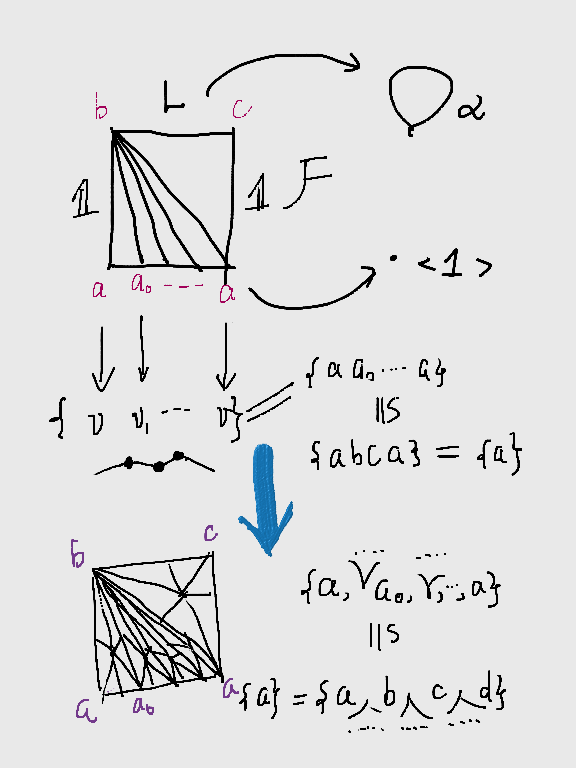
\includegraphics[width=0.9\linewidth]{pics/ch6-notes-2/L.png}
    \end{figure}
\end{proof}

\begin{remark}
    This theorem already tells us that the Edge group $E(K,v)$ is
    indepedent on the choice of base point $v$, since our polyhedron
    $|K|$ is always assumed to be path-connected.
\end{remark}

Based on this edge group, we will try to calculate more explicitly the
structure of this group. Here we provide a way to get the generators
and relations directly from the edge group.

\begin{key}
    The intuition is that the structure of this group is
    determined only by those $1$-simplexes, $2$-simplexes, and the
    equivalence relations between edge pathes. All higher dimensional
    simplexes are not relevent to this group structure.
\end{key}

We let \nomen{$L$} the subcomplex of a simplicial complex $K$. This
subcomplex $L$ is required to contain all the vertices of $K$ and such
that its polyhedron $|L|$ is path-connected and simply-connected. Can
we find such a subcomplex? The intuitive answer is yes due to the
path-connectedness nature of $|K|$. The rigorous answer needs the help
of a concept \nomen{tree}. A tree $T$ is a one-dimensional subcomplex of
$K$ whose polyhedron $|T|$ is both path-connected and
simply-connected. The following lemma affirms that we can find our $L$
to be exactly the maximal tree in $K$:
\begin{lemma}
    A maximal tree contains all the vertices of $K$.
\end{lemma}
\begin{proof}
    We first observe that a tree must exists, unless the dimension of
    $K$ is $0$ (in which case, there is entirely no need for the
    following discussions, and the lemma is still true because there is
    not even a maximal tree!). Let $T$ be a maximal tree in $K$, which
    means that if $T'$ is a tree and contains $T$, than $T'=T$. 
    The next step is simply and is expatiated on page 134 of
    \cite{book}. The idea is to grow a tree by adding more vertices,
    which is possible because $|K|$ is path-connected and a path can
    be easily turned into an edge path. Note that add a
    simply-connected space in this way will keep the space
    simply-connected, just do not add a vertices twice too creat a
    loop. 
    
    Obviously one will get a tree which is maximal and contains all
    the vertices.  Such a process also affirms that the maximal tree
    will exist (but may not be unique).
\end{proof}

\begin{ex}
    Here is the maximal tree of the triangulation of two-torus:
    \begin{figure}[H]
        \centering
        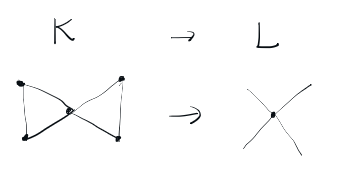
\includegraphics[width=0.9\linewidth]{pics/ch6-notes-3/ex1-maximal-tree.png}
    \end{figure}
\end{ex}

\begin{ex}
    The maximal tree is usually not unique!
    \begin{figure}[H]
        \centering
        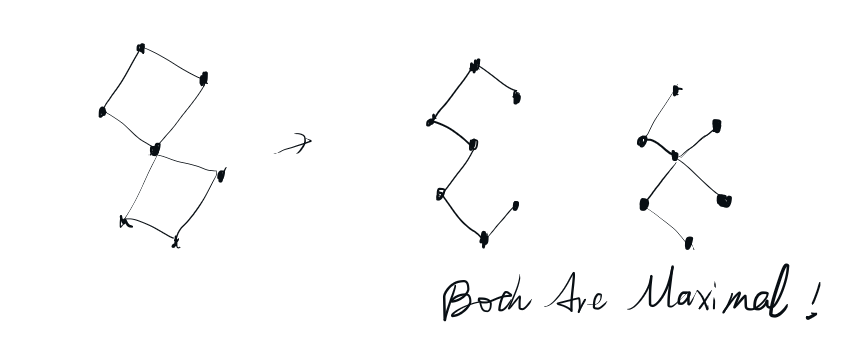
\includegraphics[width=0.9\linewidth]{pics/ch6-notes-3/ex2-maxi-tree-not-unique.png}
    \end{figure}
\end{ex}


Now since $|L|$ is simply-connected, it will not contribute to the
edge group. What contributes to the edge group is those edges that are
not in this $|L|$. This motivates us to define a new group:

\begin{defi}[$G(K,L)$]
\nomenclature{$G(K,L)$}{\nomrefpage.}
    Let $L$ be the maximal tree in $K$ (assume $|K|$ is
    path-connected). Then $G(K,L)$ is defined by generators $g_{ij}$
    for each \textbf{ordered} pair of vertices $v_i,v_j$ such that
    $\{v_i,v_j\}$ spans a simplex ($0$-simplex or $1$-simplex) in $K$.
    Those generators are subject to the following conditions:
    \begin{enumerate}
        \item $g_{ij}=1$, the identity element, if and only if
            $\{v_i,v_j\}$ spans a simplex in $L$.
        \item $g_{ij}g_{jk}=g_{ik}$ if and only if $\{v_i,v_j,v_k\}$
            spans a simplex ($0$ or $1$ or $2$ simplex) in $K$.
    \end{enumerate}
\end{defi}

\begin{ex}
    \label{ex:torus-GLKgroup}
    Again, for torus:
    \begin{figure}[H]
        \centering
        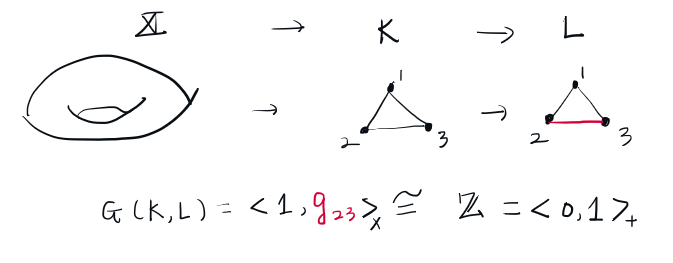
\includegraphics[width=0.9\linewidth]{pics/ch6-notes-3/ex3-L-in-triangle.png}
    \end{figure}
\end{ex}
\begin{ex}
    \label{ex:ex4-L-in-two-torus}
    And for another:
    \begin{figure}[H]
        \centering
        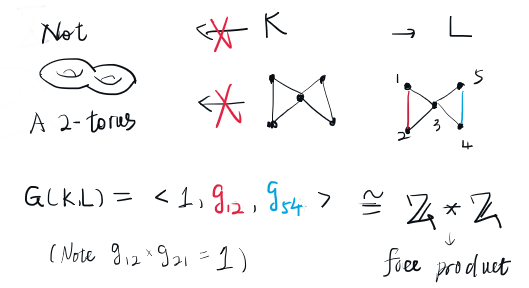
\includegraphics[width=0.9\linewidth]{pics/ch6-notes-3/ex4-L-in-two-torus.png}
    \end{figure}
    Note that this does not gives a triangulation of two-torus! 
    The reason will be explained later in
    example~\ref{ex:pi1-two-torus}.
\end{ex}
More generally, we have
\begin{thm}
    $G(K,L)\cong E(K,v)$, as a group isomorphism.
\end{thm}
\begin{proof}
    The proof in page 135 to 136 of \cite{book} constructs the
    following homomorphisms:

    $$\begin{tikzcd}[]
        G(K,L)\ar[r,"\phi",shift left] & 
            E(K,v)\ar[l,"\theta", shift left]
    \end{tikzcd}$$

    It is pretty simple to get these two maps and confirms that their
    composites are identity functions on each space.
\end{proof}

\begin{remark}
    We have now the following chain of homomorphisms:
    $$ \pi_1(|K|,v)\cong E(K,v) \cong G(K,L) $$
\end{remark}
\begin{coro}
    For any path-connected, triangulable space, its fundamental group
    is finitely presented, i.e., the fundamental group has only a
    finite number of generators and a finite number of relations.
\end{coro}

For example, we have demonstrated in example~\ref{ex:torus-GLKgroup}
that its $G(K,L)\cong \Z_2$, which is just its fundamental group.

In addition, armed with this tool, we can answer an additional
question. We want to know what is the fundamental group of two torus
connected together:

\begin{figure}[H]
    \centering
    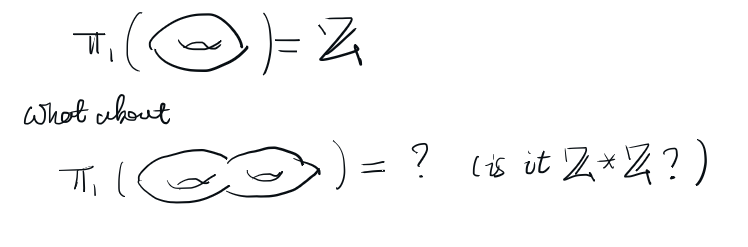
\includegraphics[width=0.9\linewidth]{pics/ch6-notes-3/pic-two-torus.png}
\end{figure}

This can be done using the following theorem:

\begin{thm}[Van Kampen's theorem]
    Let $J$, $K$ be two simplicial complexes in some Euclidean space
    which intersect in a common subcomplex, and suppose all $|J|$,
    $|K|$, $|J\cap K|$ are path-connected. Let $j,k$ be the inclusion
    maps:
    $$ \begin{tikzcd}[]
        \lvert J\cap K\rvert \ar[r,"j",hook] & \lvert J\rvert
    \end{tikzcd}$$
    $$ \begin{tikzcd}[]
        \lvert J\cap K\rvert \ar[r,"k",hook] & \lvert K\rvert
    \end{tikzcd}$$
    Take a vertice $v\in J\cap K$ as the base point. The fundamental
    group $\pi_1(|J\cup K|, v)$ is obtained from the free product
    $\pi_1(|J|,v)*\pi_1(|K|,v)$ by adding the relations
    $j_*(z)=k_*(z)$ for all $z\in\pi_1(|J\cap K|,v)$.
\end{thm}
\begin{proof}
    The proof can be found on page 137 to 138 of \cite{book}. Please
    do read the paragraph just before this theorem to get a picture of
    the proof.

    Note also that a $2$-simplex cannot possiblly cross the
    intersection part $J\cap K$. Please check why I mention this when
    reading the proof on the book \cite{book}.
\end{proof}

\begin{ex}
    \label{ex:pi1-two-torus}
    Here's how to find the fundamental group for two-torus connected:
\begin{figure}[H]
    \centering
    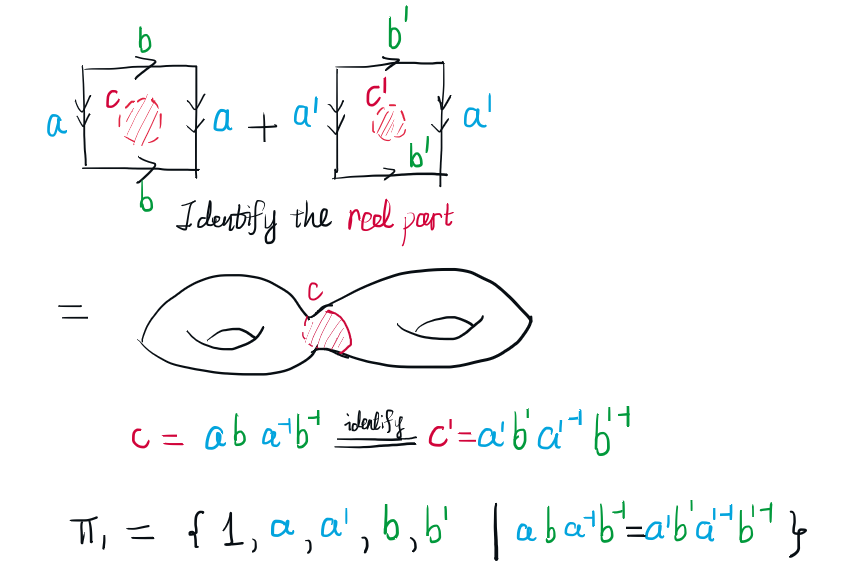
\includegraphics[width=0.9\linewidth]{pics/ch6-notes-3/ex-pi1-two-torus.png}
\end{figure}
    The result confirms that the triangulation of a two-torus is as
    simple as in example~\ref{ex:ex4-L-in-two-torus}.
\end{ex}

\begin{ex}
    Next we consider the projective space $\R P^2$, the space is
    homeomorphic to half the sphere $S^2$, with the antipodal points
    on the boundary identified:
    \begin{figure}[H]
        \centering
        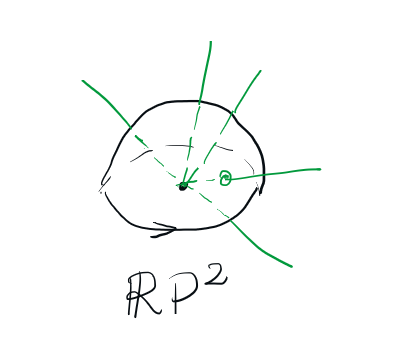
\includegraphics[width=0.4\linewidth]{pics/ch6-notes-3/rp2.png}
    \end{figure}
    Then it can be regarded as a 2-disc with it boundary attached to
    the boundary of a M\"obius strip. This construction will tell us
    that the fundamental group of $\R P^2$ is $\Z_2$.
    \begin{figure}[H]
        \centering
        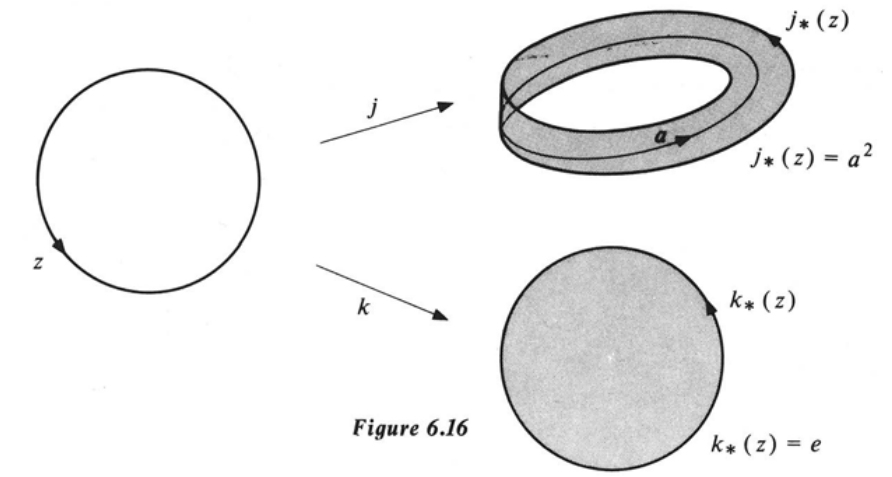
\includegraphics[width=0.8\linewidth]{pics/ch6-notes-3/rp2-pi1.png}
        \caption{Page 139, Fig 6.16 of \cite{book}}
    \end{figure}
\end{ex}



\section{Anchor}
\label{sec:Anchor}

\begin{thebibliography}{1}
    \bibitem{book} M.A. Armstrong. Basic Topology. 2ed.
    \bibitem{Singer.Thorpe} I.M. Singer, J.A. Thorpe. Lecture Notes on
    Elementary Topology and Geometry. UTM.
\end{thebibliography}
\printnomenclature
\section{License}
The entire content of this work (including the source code
for TeX files and the generated PDF documents) by 
Hongxiang Chen (nicknamed we.taper, or just Taper) is
licensed under a 
\href{http://creativecommons.org/licenses/by-nc-sa/4.0/}{Creative 
Commons Attribution-NonCommercial-ShareAlike 4.0 International 
License}. Permissions beyond the scope of this 
license may be available at \url{mailto:we.taper[at]gmail[dot]com}.
\end{document}
